%!TEX root = ../thesis.tex
%*******************************************************************************
%****************************** Second Chapter *********************************
%*******************************************************************************

\chapter{Trends in Deforestation and Environmental Policy in Maranhao, Brazil}

\ifpdf
    \graphicspath{{Chapter2/}{Chapter2/}}
\else
    \graphicspath{{Chapter2/}{Chapter2/}}
\fi


\begin{abstract}
This study investigates deforestation trends in the Brazilian \textit{Cerrado} region in Maranhao, Brazil, which provides a unique natural experiment in that there were spatially hetereogenous environmental policies to combat deforestation in place. The analysis applies the non-linear estimation approach of Generalized Additive Models (GAMs) on satellite data derived measures of deforestation, where validation is conducted using features of neural networks. The GAMs confirmed that deforestation is related to climatic factors in that increased during high levels of precipitation and low levels of solar incidence.  More importantly, the results revealed that there are substantially differences in trends between seasons across regions according to their policy distinction. This was further substantiated by showing that deforestation happened during both seasons for settlements which were not target of the environmental policy, but only during the rainy season for the protected areas, likely due to the lower rate of remotely sensed detection during cloud cover.\\
\noindent{\bf Keywords:} Deforestation trends, Generalized Additive Models, Remote Sensing Analysis.

\end{abstract}


\section{Introduction}
\label{S:1}

%trends are likely to influence health care delivery services in the future for many reasons

%Understanding the dynamics of land-use and land-cover (LUCC)\footnote{A long the lines of the Land-Use and Land-Cover Change (LUCC) project of the International Geosphere-Biosphere Program (IGBP) and International Human Dimensions Program (IHDP) on Global Environmental Change \citep{GEIST}. In the past, land-use and land-cover change was a hybrid category. Land use denoted the human employment of the land and was studied largely by social scientists and land cover denoted the physical and biotic character of the land surface and was largely studied by natural scientists \citep{MEYER}} has increasingly been recognized as one of the key research imperatives in global environmental change research. The growing recognition of the contribution of forests to climate change has created new momentum in the fight against tropical deforestation and forest degradation \citep{CAROLE2013}.

Tropical deforestation is relatively a modern event that only gained momentum in the second half of the $20^{th}$ century. As a matter of fact, the considerable deforestation observed globally during 1990-2010 was almost entirely confined to the tropical regions \citep{CULAS11}.  In this regard, the Brazilian Cerrado is perhaps the biome which has arguably been most affected by human occupation over the last three decades, mainly due to the increasing pressures for opening up of new areas for the production of meat, grains and ethanol, mostly at the sacrifice of forested areas \citep{mma_2018, bayma_sano_2015}. Importantly, the Brazilian Cerrado has also been subject to spatially and temporally heterogeneous environmental policies discouraging such deforestation.  Understanding what role such interventionist policies may have played in observed trends in deforestation could potentially provide a platform with which to assess future possible scenarios of deforestation in the Cerrado biome and the Amazon forest in general \citep{boyd_2013}. In this paper we use remote sensing data and non-linear models to model the trends of deforestation and its underlying drivers in the \textit{Cerrado} region in the Brazilian state of Maranhao using the non-linear modelling approach of Generalized Additive Models (GAMs). 

Arguably, the state of Maranhão provides a particularly interesting context within which to study trends in deforestation and the possible role of environmental policy.  More specifically, Maranhão is divided by an artificial line that separates it in two parts: the Legal Amazon Maranhão and the Cerrado Maranhão. This division, occurring approximately 44$^{\circ}$ west of the meridian, was established in 1953 due to the necessity to plan economic development in the region. This scenario provides a unique natural experiment of deforestation in the Legal Amazon Maranhao (LM) and Cerrado Maranhao (MA) since the former has been subject to fundamentally different environmental policies compared to the latter.\footnote{The Legal Amazon is an area that corresponds to 59$\%$ of the Brazilian territory and encompasses all eight states (Acre, Amapá, Amazonas, Mato Grosso, Pará, Rondônia, Roraima and Tocantins) and part of the State of Maranhão (west of the meridian Of 44ºW), totalling more than 5 million km$^{2}$ \citep{IPEA2}.} More specifically, the tropical forest in the Legal Amazon Maranhao is under a surveillance environmental policy, called DETER, which detects deforestation or fire incidence  in the region using satellite data and informs the occurrences to the environmental police (IBAMA in Portuguese) so that they can fine or arrest the responsible persons \citep{IBAMAwebsite}. In contrast, DETER is not applicable for the other biomes in the Maranhao state.\footnote{The DETER is a rapid survey of alerts of changes in forest cover in the Legal Amazon made by National Institute os Spatial Research (INPE in Portugues) since May 2004, with data from Terra's MODIS sensor, with a spatial resolution of 250 m. DETER was developed as an alert system to support the environmental police to curb illegal deforestation. With this system, it is possible to detect only changes in the forest cover with an area larger than 25 ha. Due to cloud cover not all changes are identified by DETER. The lower resolution of the sensors used by DETER is compensated by the daily observation capacity, which makes the system an ideal tool to quickly inform the inspection bodies about new changes DETER operates daily and delivers deforestation alert maps to environmental policy in a five days after the date of the MODIS image \citep{inpe-deter_2018}.} We use this spatial division to determine how deforestation trends may have been different being the Legal Amazon Maranhao and Cerrado Maranhao.

Our use of non-linear modelling for the task at hand derives from the recognition by recent previous research that most ecological and climatic data represent complex relationships and thus that non-linear models, such as GAMs, may be particularly suited to capture confounding effects in trends; see \citep{alkemad_1998,BELL_2015,JOYE_2015,LUSK_2016,SADAT_2016,HALPERIN_2016, SANTOS_2017,TAPIA_2017, LIU_2018,MORENO_2018}. However, a review of the literature shows that such models have only been used sparsely to study deforestation. For example, \citet{COHEN_2008} modelled how deforestation affected incidence rates of a disease in Cuba. Also, \citet{GREEN_2013} used a binomial GAM model to account for forest and habitat losses in protected areas on the Eastern Arc Mountains of Tanzania. More recently, \citet{BEBBER_2017} studied the impact of protected areas on global carbon emissions in America, Africa and Asia. For Brazil, \citet{MENDES_2012} observed the relationship between deforestation, corruption, and economic growth in the region of Legal Amazon, in Brazil. Here we apply a GAM with a negative binomial distribution and logarithmic link function. To capture deforestation we construct monthly time series from remote sensing sources (MODIS), given that high temporal resolution satellite products are particularly suitable to obtain detailed knowledge about the seasonal cycles of vegetation in biomes with strong seasonal contrast, such as the Cerrado biome and Ecotone forest \citep{bayma_sano_2015}. Our climatic covariates are derived from data from meteorological stations. 

%For handling spatial datasets, ArcMap 10.4.1, ArcPy 10.4.1, and the extensions Geostatistical Analyst, Spatial Analyst and Spatial Statistics from ArcToolbox \citep{esri_2016,arcpy_2016}, and MATLAB R2017a with Statistics and Machine Learning and Image Processing Toolbox \citep{matlab_2017} was extensively used. For statistical analysis and modelling, R \citep{R_2018} and several packages specially 'MASS'\citep{MASS_2002}, 'mgcv' \citep{Wood_2003, Wood_2004, Wood_2011, Wood_2017} and 'gratia' \citep{Gavin_2018} were considered.

%In the results, the GAMs confirmed that deforestation is related to year and climatic variables, but also revealed that there is substantially difference of trends between seasons and sub regions (Legal Maranhao and Cerrado Maranhao). These results show that it does seem that deforestation in the Amazon region (LM) was transferred during the dry season to the Cerrado region (MA). It is not possible to check if this shift also happened during the raining season because both regions presented positive increment for deforestation. There appears to be no spillover effect from the environmental enforcement executed in the LM region to the MA region. One plausible proof is that deforestation remained during both seasons with distinct cycles. 

%With these results, three possible outcomes emerges: i) since the region is a transitional zone, the two areas don't differ in biota aspects. In a sense, anthropic actions were responsible for apparent changes in the deforestation trends and, these changes ii) happened during high levels of precipitation and low levels of solar incidence which in turn shows that, in general, cloud cover might be a benefit for clear-cutting practices, keeping in mind that iii) the artificial line divides the two regions but many of the political boundaries of municipalities remain in both sides of the region (MA and LM), which could interfere in the deforestation path between the seasons.

The results from our GAMs revealed that for the Legal Maranho region most of the deforestation happened during the rainy season, while in the unprotected Cerrado Maranhão deforestation occurred in the dry season as well.  The fact that precipitation and solar incidence also played an important role in deforestation in the rainy season in the Legal Maranho region suggests that cloud cover may have acted as an impediment to infringement detection via satellites, as is done in the DETER program. We further substantiated this claim by showing that for settlements that were not the target of environmental policy deforestation mainly took place during both seasons as well.     


%Several studies focused on deforestation trends in Brazil Amazon and Cerrado taking into consideration climatic and socioeconomic factors \citep{shukla_1990, skole_1993, morton_defries_2006, costa_pires_2009, nepstad_2008, nepstad2_2014}\footnote{For a detailed bibliometric analysis of deforestation trends, see \citet{Benavent_2018}.} However, most ecological and climatic datasets present a 

%Amazon Maranhao and Cerrado Maranhao show a decreasing trend which imposes the main questions of this study. Is the decreasing deforestation trend in Amazon Maranhao during 2000 to 2017 displaced to the Cerrado Maranhao? And, is there a spillover effect from the environmental policy in the decreasing trend in deforestation on the Cerrado Maranhao? 


%Monthly data

%New technique applied to deforestation

\section{Study Context}  %mudar o titutlo
\label{S:2}
\subsection{Study Location} %mudar o titutlo

%Paragrafo introdutorio com dados demograficos, sociais economicos. Explicar a diferente estrutura da regiao ML/MA

Maranhão, or \textit{'flowing river'} in the indigenous language \citep{girardi_2015}, is one of the ten largest States of Brazil with more than 330 thousand square kilometers and located in the northeast part of Brazil. However, while it is considered one of the richest regions in biodiversity in the country \citep{BATISTELLA_2014}, it has historically ranked among the states with the worst social and economic indicators \citep{CELENTANO_2017}.  The State's political boundaries encompass natural hydrological barriers, where within these borders 64.1\% of the area of the territory is in the Cerrado/Savana biome, 34.8\% in the Amazon biome, and only 1.1\% in the \textit{Caatinga} biome \citep{STELLA_2011}. The Cerrado represents the largest ecosystem in Maranhão, and is located from the Northeast to the southern region of the State, covering about 60\% of its surface, occurring in approximately 55 of the total 217 municipalities. Of these, 23 are almost exclusively covered by this type of vegetation \citep{BATISTELLA_2013}. 

In terms of vegetation, in the centre of Maranhão there is a contact area between the Amazonian and Cerrado biomes of around 21.228$km^2$, where it is possible to observe a mosaic of savanna vegetation physiognomies concomitant with the ombrophilous forest formations (open and dense forest). This area is known as an Ecological Tension Zone (ETZ) of Maranhao and is home to a transitional vegetation which usually occurs with intermediate characteristics of the two formations, with species common and distinct to both, providing great biodiversity \citep{rossatto_2013}. In Maranhão Cerrado it is also possible to distinguish between ecotonic areas and the presence of secondary vegetation in the central region of the state. Ecotone is defined as the transition area between two or more distinct habitats or ecosystems, which may have characteristics of both or their own. Secondary Vegetation includes the various stages of natural succession in areas where there was human intervention for land use, whether for mining, agricultural or livestock purposes, or discharging the primary vegetation \citep{SANTOS-FILHO_2013}. 

There is a strong debate over the definition of the ecotone forest and secondary vegetation in the state of Maranhão. Considering the Cerrado/savanna territory, almost 10\% represents the transition and secondary forest. \citet{REIS_2010} state that the Cocais Forest (\textit{"Mata dos Cocais"} in Portugues) is considered a characteristic landscape of the State, although it develops in the transition between several biomes. The authors pointed out that the Cocais Forest associates with the open fields, towards the North, with the Cerrado vegetation to the South and East, and gradually joins the forest towards the west. 

%In terms of population, Maranhão is the 10th more populated state with a resident population of ${\sim}$ 6mi in 2015, which represents 3.4\% of the inhabitants living in Brazil. In addition, Maranhão has the highest percentage of people residing in rural areas comparing to other states however the economic activities are centred in Services (70\%), Industry (19\%) and Agriculture (11\%) \citep{imesc_2015}.




%falar da regiao tropical do maranhao

%The Amazon tropical forest is the largest biome in Brazil, occupying almost half of the national territory. Dominated by hot and humid climate and well distributed rains during the year, this biome has the characteristic vegetation of tall trees and forests periodically and permanently flooded. In Maranhão, the rainforest is formed by dense forest (Ombrophylous Forest), open forest (Ombrophylous Forest) and seasonal forest (Semidecidual Forest) corresponding to more than 60 thousand square kilometers \citep{BATISTELLA_2013}. 

%The characteristic of the dense forest is associated to tropical climatic factors of high temperatures (averages of 25$^{\circ}$C) and high precipitation, well distributed during the year which determines a practically no dry period. In Maranhão, this region occurs in 6.45 \% of the state, located mainly in the most western portion of the state. The open forest presents different floristic forms that alter the ecological aspects of the dense forest, giving hence the name adopted, besides climatic gradients with more than 60 dry days per year, configuring a dry season. This forest region encompasses 0.18\% of Maranhão and also situates at the Maranhão's western portion. The ecological concept of the seasonal forest type is established as a function of the occurrence of seasonal climate, which determines semideciduous forest foliage. In the tropical zone, it is associated with the region marked by severe winter droughts and intense summer rains. In Maranhão, this type of forest covers 12.30 \% of the state, mainly towards the centre portion of the state \citep{BATISTELLA_2013, SPINELLI_2016}. 


%falar da caatinga 

%Although having a small percentage in the State (1.1\%), the \textit{Caatinga} biome is considered the most bio-diverse semiarid region in the world, characterised by shrubs with twisted branches and deep roots and cacti. In Maranhão, the \textit{Caatinga} domain presents a strong climatic irregularity, and its meteorological values are the most extreme in the state: the strongest sunshine, the lowest cloudiness, the highest thermal averages between 25$^{\circ}$ and 30$^{\circ}$ C, the highest evaporation rates and, especially, the lowest pluviometric indices, around 500 to 700 mm annually, with great spatial and temporal variability \citep{LOIOLA_2012}.

%falar do cerrado 

%The Cerrado Biome in several regions of Brazil is bordered by other plant formations, being characterised by being the second largest Brazilian biome in territorial extension, being surpassed only by the Amazon \citep{BATISTELLA_2013}. 


%[PARAGRAFO PARA FAZER LIGACAO COM O SUBSECTION]



%\subsubsection{Ecotone Forest and Secondary Vegetation in Maranhao}

%Authors discuss the difficulty of delimiting forest areas in transitional and / or ecological tension regions, mainly Cerrado - Amazon Forest due to the innumerable indentations and interpenetration of savanna formations in the territory of the Legal Amazon. Areas with these characteristics can be found in the states of Amazonas, Mato Grosso, Pará, Tocantins and, specially, in Maranhão.



%Differently, \citet{azevedo_2002} assigns the Cocais Forest as a secondary type of vegetation present in the two types of forests in Maranhão: the humid one, and the deciduous (periodic exchange of foliage). The author explains his assumption based on historic reports demonstrating that the ecosystem used to be different in that region. Officially, the Cocais forest is considered an open forest transition with palm trees \citep{ibge_1992}. \citet{RIBEIRO_2008} have also designated Cocais Forest as one of the features that occur in the Cerrado environment. 

More recently, \citet{GARCIA201716} studied part of the Maranhao region and defined forest as a combination of riparian forest, transitional forest, and Cerrado woodland - the latter defined as having higher tree density and Cerrado, representing physiognomies with a wood layer but lower tree density. Their results showed intense conversion and fragmentation of native vegetation and, consequently, the impoverishment of the quality of native cover, reassuring the possibility of conducting studies considering ecotone forest,such as \textit{Mata dos Cocais}, as a transition forest instead of secondary vegetation.


As noted in the introduction, in addition to the natural barriers, Maranhão is also divided into two parts: the Legal Amazon Maranhão and the Cerrado Maranhão, with 209 municipalities located in the latter and 138 municipalities in the former. This division occurs approximately 44$^{\circ}$ west of the meridian and was established in 1953 in order to plan the economic development of the region comprised of the tropical forest areas of Maranhao state.  We depict this delineation in Figure \ref{fig:delimitacao}

\begin{figure}[H]
  \centering
  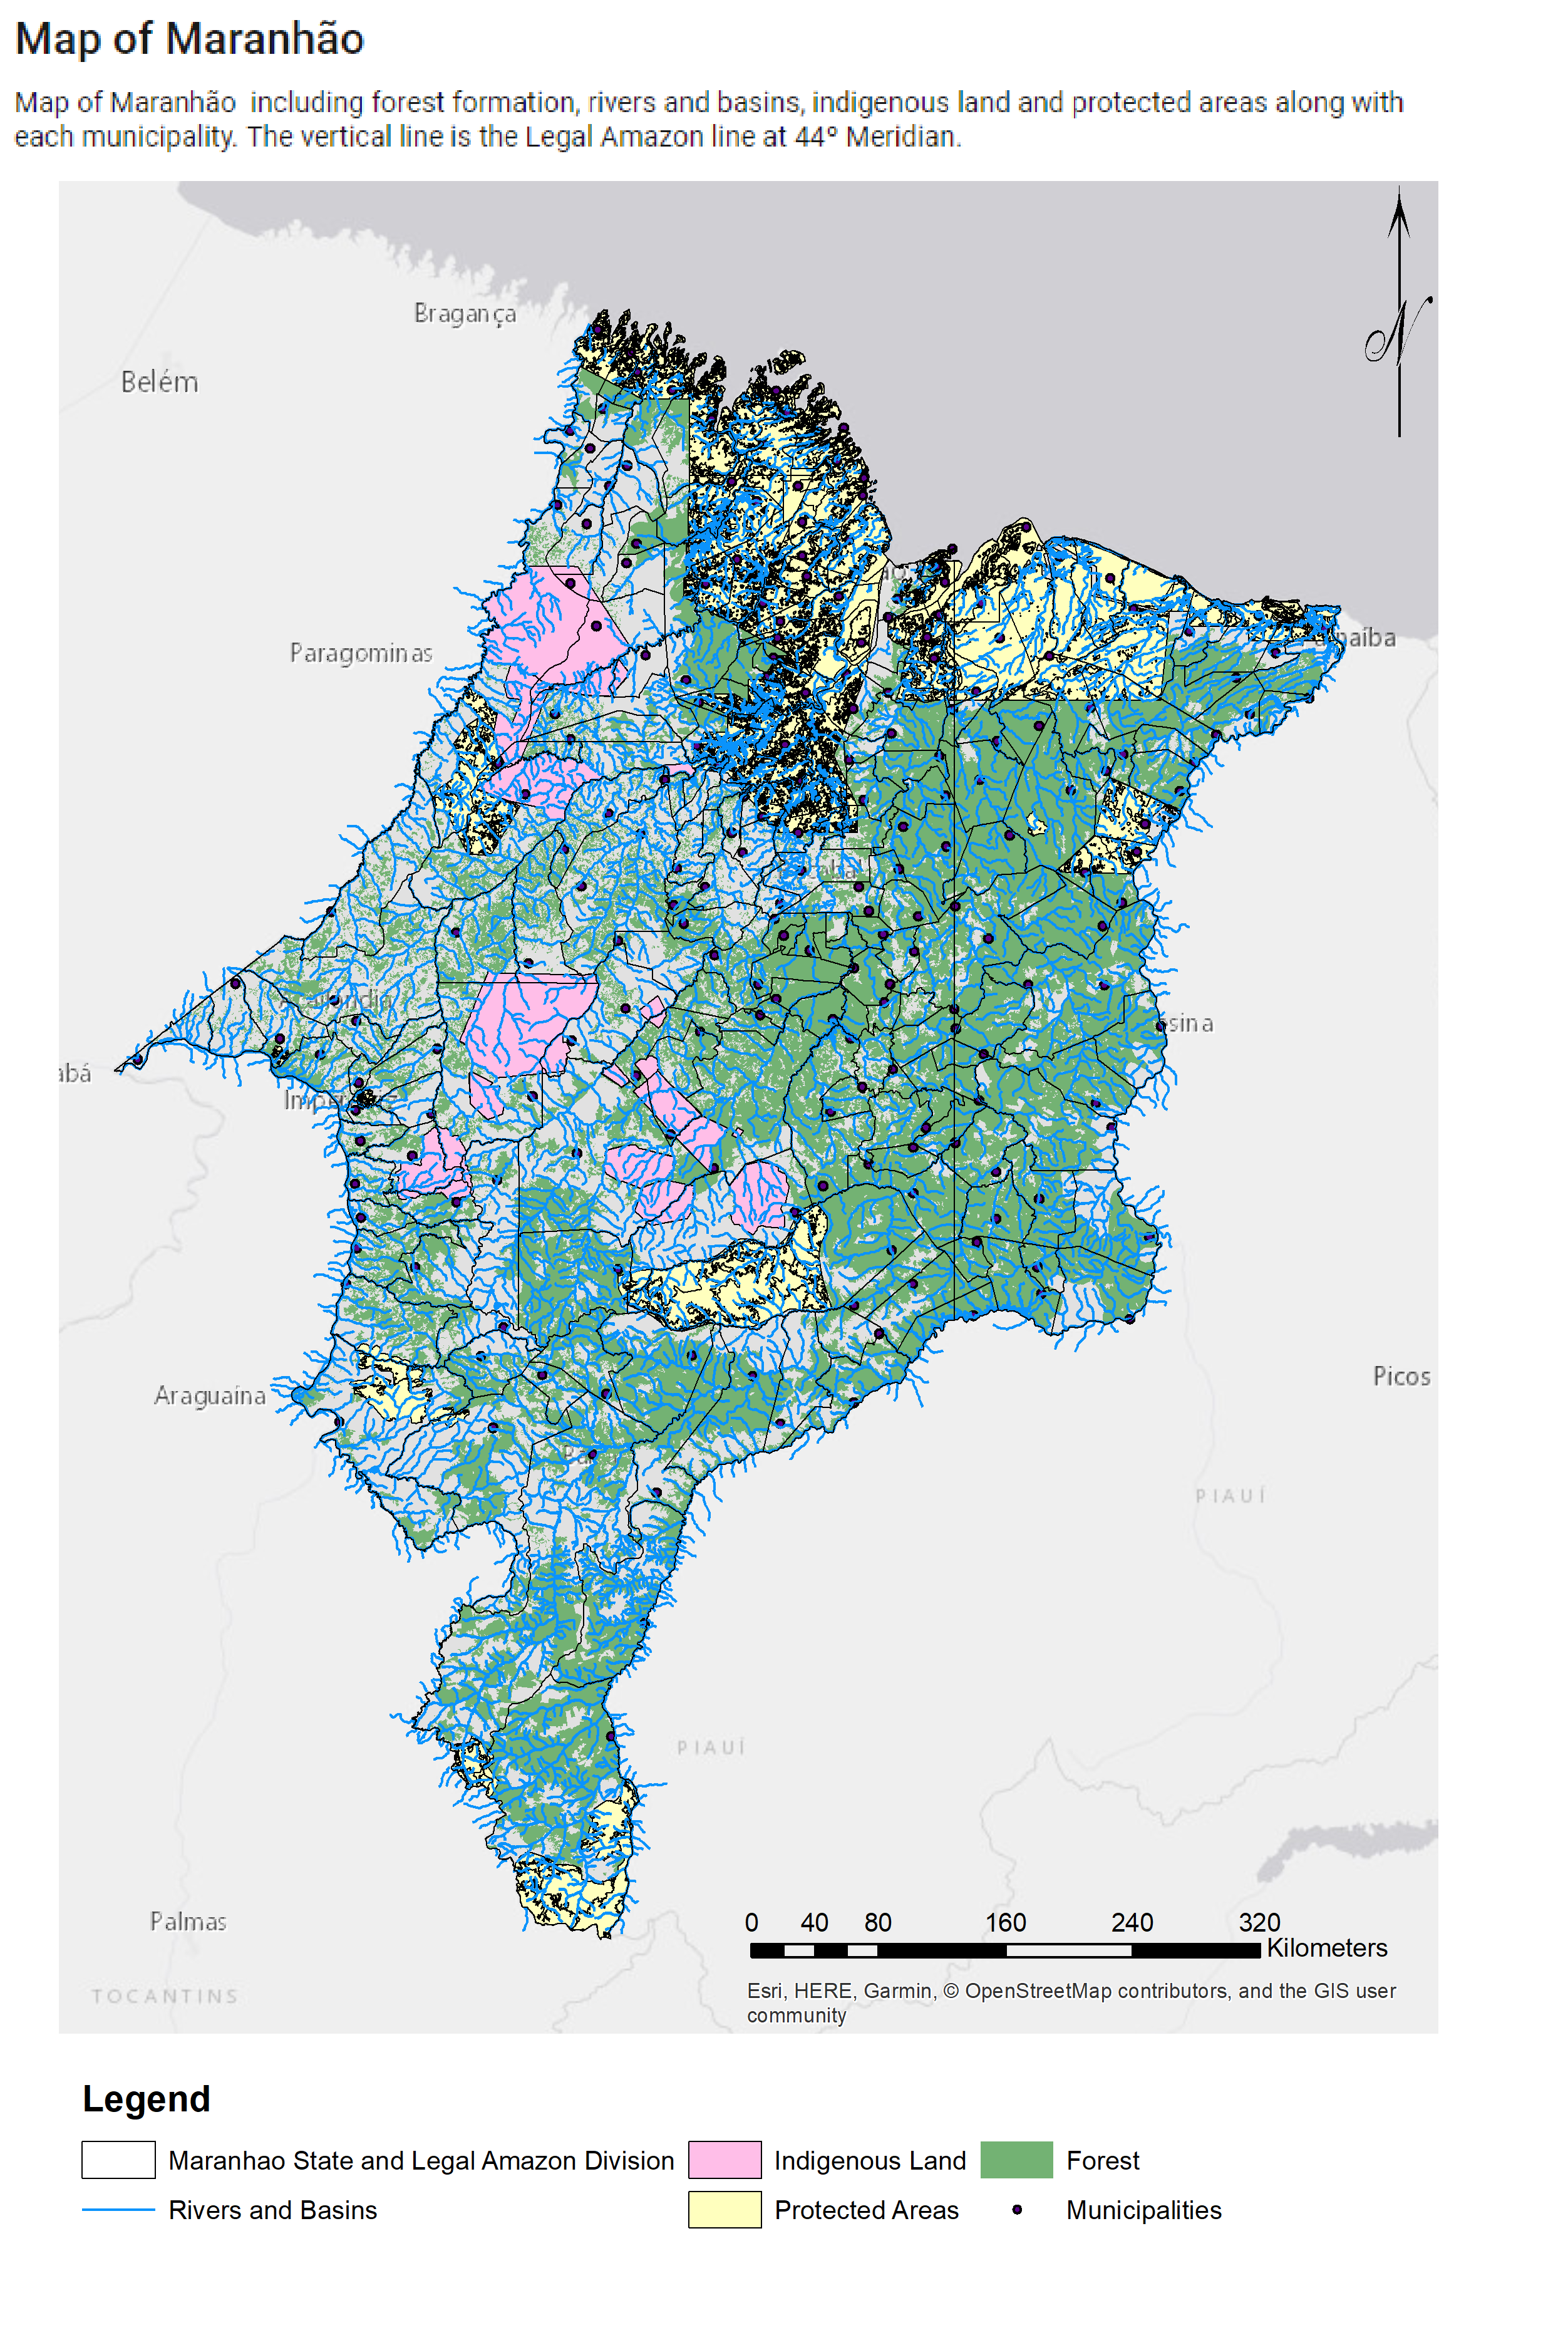
\includegraphics[width=0.9\textwidth, inner]{MaranhaoState2.png}
\caption{Source: \citep{MMMAwebsite,nugeo_2018,embrapa_2018}.}
\label{fig:delimitacao}
\end{figure}

%COLOCAR QUE EXISTE UM EMBATE PARA O TIPO DE VEGETACAO SECUNDARIA NO MARANHAO - SE EH ALGO ANTROPICO OU NATURAL POR PARTE DA REGIAO. VER O ARTIGO DE SOARES-FILHO 2013.


%Com base nos relatos de antigos viajantes de que regiões constituintes da Zona dos Cocais, como é atualmente denominado o ecótono presente em parte do território dos estados do Piauí e do Maranhão, continham várias populações de palmeiras, mas, especialmente em território maranhense, prevalecia uma floresta com características da pré-Amazônia e considerando os diferentes trabalhos e ensaios com várias espécies de palmeiras e suas respectivas propriedades no processo de recrutamento e sucessão ecológica, pode-se supor que a maciça concentração de grandes populações encontradas na região atualmente, seja reflexo de um intensivo processo de degradação das florestas originais com diferentes finalidades, partindo-se desde a exploração de territórios para pasto e agricultura, quanto ao extrativismo de plantas típicas das florestas presentes na região. O resultado desta degradação deixa evidente que, dentre estas espécies de palmeiras, o babaçu é uma das plantas mais expressivas e eficientes da comunidade pioneira.

\subsection{Deforestation in Maranhão}

%Studies of deforestation seem to vary from place to place. In Brazil, and specially Maranhão, deforestation happens depending on the status of development and welfare of the citizens in determining the extent of the forest loss. The requirement for income and economic growth results in growing demand for agricultural and forest derived products, like soy, timber and beef. The main causes of deforestation are assumed to be acting aggregated and the government finds these are the easiest and the most accessible ways of responding to their increasing economic pressures \citep{GEIST,CULAS11,CELENTANO_2017}.

%EXPLICAR A RAZAO PELA QUAL TEM DESMATAMENTO NO MARANHAO
Large-scale deforestation in the Maranhão Amazon forest began in the 1960s, when the military government promoted the occupation of this territory through the construction of highways and provided incentives for large farming projects on public lands and logging centres. In the 1980s, with the implantation of the iron mining project in the in the neighbouring state of Pará (Carajas Project), a railroad linking the mine to the port in Maranhão was built. Moreover, many pig iron facilities were installed in the Maranhão Amazon region, demanding large quantities of charcoal, which increased the pressure on forest resources \citep{CELENTANO_2017}.

%Colocar graficos 
%COMO EH ESSE DESMATAMENTO COMPARADO COM A AMAZONIA LEGAL E COM O RESTANTE DO CERRADO

While many existing studies have focused on the Amazon tropical forests \citep{PFAFF,PFAFF2,HAMMIG,GEIST, GEIST2, LAMBIN2,PFAFF3,ZAMBRANO,KUIK,COE,SOLER,NEPSTAD,ARIMA,PATZ,CULAS11,RICHARDS,RICHARDS2,CELENTANO_2017} due to the fact the ample environmental information was available through specific environmental policies, such as DETER, studying the Cerrado biome and, consequently, transition forests remains precarious. The first obstacle in monitoring the Cerrado biome is due to the high heterogeneity of the forests (open and dense forest, for example) which are substantially influenced by the climatic seasonality \citep{bayma_sano_2015}. The second challenge is related to the fact that there is no environmental policy in place to prevent rampant deforestation.  Nevertheless, in the context of the Amazon region, it is arguably crucial to understand the dynamic of Cerrado and its potential to influence adjacent forests of Amazonia since it provides a valuable endpoint from which climate and anthropogenic related aspects in the Amazon forest my be better understood (see Figure \ref{fig:defAmazonMA}).  

%In this sense, the Cerrado is the Brazilian biome most affected by human occupation in the last three decades, mainly due to the increasing pressure for the opening of new areas for the production of meat, grains and ethanol, which puts the survival of many species and the integrity of their habitat in risk \citep{mma_2018, bayma_sano_2015}. 


%Considered a transitioning state between semiarid and tropical environment, Maranhão's Cerrado figures the third position when comparing the amount of forest cleared in absolute values demonstrating that the end-point of Amazon forest is at risk (Figure \ref{fig:defAmazonMA}).  

\begin{figure}[H]
  \centering
  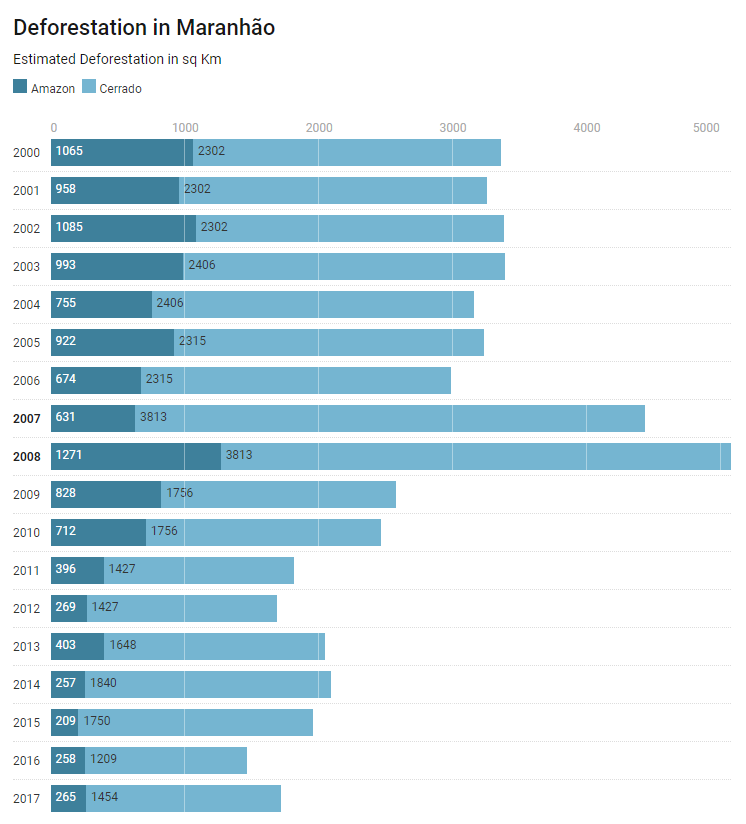
\includegraphics[width=1\textwidth, inner]{chartMA.png}
\caption{Source: \citep{MMMAwebsite}.}
\label{fig:defAmazonMA}
\end{figure}

%SERIA BOM COLOCAR O TREND DE DESMATAMENTO DE HANSEN PARA A PARTE QUE NAO TEM DADOS DO PRODES.

In the past many aspects have arguably contributed significantly to deforestation in the Cerrado Maranhao, such as the agricultural occupation of the Cerrado biome and the unconstrained use of mechanisation, propitiated by the predominantly flat relief of the region and the existence of good depth soil conditions and good water supply, making it possible to practice rainfed agriculture \citep{bayma_sano_2015}. In contrast, more recent forest losses  have been due to settlement projects, illegal logging, pasture, subsistence agriculture and commodities \citep{CELENTANO_2017, costa_2018}, and these drivers are deeply connected to the process of the state's development. More precisely, during the 40's, almost 85\% of the population was living in rural areas with low rate of population density (3,81). At that time, Maranhao had more than 200.000 km$^{2}$ uninhabitated, which included transition forest, Cerrado, and pre-Amazon forest. This "territorial gap" (/textit{fundos territoriais} in Portuguese) favoured the creation of several settlement projects along with the creation of federal roads and the Carajas railway project \citep{ferreira_2008}. Moreover, the increasing global demand for commodities affected the economic region significantly. For instance, fiscal incentives increased the production of soy, where the planted area increased from 42,6 km$^{2}$  in 1983/84 to 3,940 km$^{2}$ in 2004/05. The subsequent ecological tension zone coincides with the Brazilian agricultural frontiers, known as the deforestation arc, and is an area of intense exploitation. \footnote{The expansion of soybean cultivation in Brazil has shifted the
agricultural frontier to an area  known as MAPITOBA. This area includes the states of MAranhão,PIauí, TOcantins, and BAhia,, and has maintained its expansion across the Cerrado This led to deforestation and degradation, conservation conflicts and conflicts over land, increased burning, and displacement of traditional populations \citep{mustin__2017}}

%Despite the rich diversity in the three explained biomes, Maranhão is the state of the Legal Amazon that presents the lowest degree of occupation of the area with protected areas. The number of endangered, rare and endemic species in the most varied groups of animals and plants attest to the biological importance of the region, not only for the State of Maranhão, but for the country as a whole \citep{MARTINS_2011}. Only during the 2000s Maranhao invested an effort on environmental policies through the creation of conservational units, indigenous land titling and environmental policies in which helped to decelerate the deforestation path in the Amazon Maranhao.

%\subsubsection{The trend of deforestation in Maranhão}

As can be seen from the graph \ref{fig:defAmazonMA}, deforestation in the Amazon biome of Maranhao has decreased over the years. Great part of this reduction is likely due to protectionist policy enforcement in the region. In this regard, the national environmental policy established in 2004 involved the creation of the Action Plan for the Prevention and Control of Deforestation in the Legal Amazon (PPCDAm in Portuguese). In order to control land use and prevent further deforestation, the PPCDAm  also included the satellite-based monitoring programme called DETER, which alerts in real time the environmental police of illegal logging and deforestation. Importantly, until July 2018 there was no systematic satellite monitoring program for the other parts of Maranhao, such as the transitional forest of Cerrado and \textit{Caatinga}. But, in August of the same year, the National Institute of Spatial Research (INPE in Portuguese) together with several other institutions published an annual dataset covering 18 years of Cerrado biome deforestation and with this data it was possible to show the trends of deforestation in the Cerrado biome of Maranhao. As shown in Figure \ref{fig:defAmazonMA}, deforestation in great Cerrado, which includes the transitional forest, has been two times higher than in the Amazon region of Maranhao.

%Both areas, notwithstanding, show a decreasing trend according to official sources which imposes two questions questions to this study: 1- Is the decreasing deforestation trend in Amazon Maranhao during 2000 to 2017 displaced to the Cerrado Maranhao? Following the first question, 2- Is there a spillover effect from the environmental policy in the decreasing trend in deforestation on the Cerrado Maranhao? By applying an advanced technique and an alternative dataset and method, this study aims to be able to answer these questions.  

%Monthly data

%New technique applied to deforestation

\section{Material and Methods}
\label{S:3}
\subsection{Remote Sensing}  %mudar o titutlo

%Anthropic activities combined with natural events are significantly altering the Earth's land cover causing global climatic changes. When considering vegetation mapping for forest cover loss and forest regrowth path, traditional methods such as field surveys are time consuming, date lagged and generally too expensive. Over the past four decades, a feasible alternative considered by researchers and specialists is to apply remote sense technology and subsequent image analysis. 

The use of satellite time series along with statistical analysis can be helpful in understanding the characteristics of vegetation dynamics.  More precisely, since vegetation has a unique spectral feature (e.g., reflectance) it is possible to identify its unique characteristics from an optical remote sensor on a satellite. In such vegetation mapping, incorporating the spectral radiances in the red and near-infra-red regions into the spectral vegetation indices (VI) gives the possibility to estimate  forage  quantity  and quality  of  grass  prairie, for example \citep{xie_sha_yu_2008}. 
Earlier studies coarse spatial resolution data from the Advanced Very High Resolution Radiometer (AVHRR) was used to mainly monitor land cover changes at regional and global scales, however, since 2000, the availability of Moderate Resolution Imaging Spectroradiometer (MODIS) data with superior features relative to AVHRR has provided an improved basis for regional and global mapping \citep{huang_2014}.
%For instance, in 1999, a group of researchers around the world created the Global Land Cover 2000 (GLC2000) project extracting data from 1-km SPOT4-VEGETATION  imagery.\footnote{For the dataset, see http://www-gvm.jrc.it/glc2000/} After two years, US-NASA  released the  database  of  global  MODIS  land  cover  based  on  monthly composites from MODIS sensor for the period between January  and  December  2001 \citep{xie_sha_yu_2008}.\footnote{For the dataset, see http://duckwater.bu.edu/lc/mod12q1.html}

%In general, the  selection of  images  acquired  by  adequate sensors is largely determined by the mapping objective and accuracy, the cost of images, the climate conditions, such as a cloud-free image, and the technical issues that arise from interpretation and suitability.

%Images with low resolutions may be adopted only when the high level of vegetation classes are to be identified, while the images with relatively higher resolutions are used for fine-detailed classifications of vegetation. Also, from the mapping scale point of view, vegetation mapping at a small scale usually requires high-resolution images, while low-resolution images are used for a large-scale mapping. In the field of vegetation mapping, the most commonly applied sensors in decreasing spatial resolution order include NOAA–AVHRR, MODIS, Landsat (mainly TM and ETM+), SPOT, IKONOS  and QuickBird \citep{xie_sha_yu_2008}.\footnote{A detailed summary of satellites, sensors and databases relevant to vegetation can be found in \citet{horning_2010}.}




\subsubsection{MODIS}

%Falar do satelite MODIS e dos seus produtos

The MODIS sensor is flown on two spacecrafts. The Terra satellite is on an AM overpass, whereas the Aqua platform provides complementary observations in the afternoon. The instrument on-board NASA’s Terra satellite is a scanning radiometer system with 36 spectral bands, extending from the visible to the thermal infrared wave-lengths, and has a viewing swath width of 2330km by 10km. The Terra orbital configuration and MODIS viewing geometry produce full global coverage every one to two days, except for the equatorial zone where the repeat frequency is approximately 1.2 days \citep{zhan_2002, setiawan_2014}. The high temporal resolution of MODIS is a determining factor in phenological studies and spectral discrimination, and can be used to obtain detailed knowledge about the seasonal cycles of vegetation in biomes with strong seasonal contrast, such as the Cerrado biome and Ecotone forest. 

%The first seven bands are designed  primarily  for  remote  sensing  of  the  land  surface with  spatial  resolutions  of  250m  (Bands 1-2), 500m (Bands 3-7), and 1000m (Bands 8-36). Note that while the bands are commonly referred to as 250m and 500m, the actual resolution of the grids is 236 and 472m at the equator. 


%In addition, MODIS data is in a ready-to-use, atmospheric corrected, cloudless, and geo-referenced format.

Of the many data products derived from MODIS observations, we use two extensively used here: MCD12Q1 and MOD13Q1. The MODIS Land Cover Type Product (MCD12Q1) provides 13 science data sets (SDSs) that map global land cover at 500m spatial resolution at annual time steps for six different land cover legends from 2001-2016. In contrast, the MCD12Q1 product is created using supervised classification of MODIS reflectance data and includes 5 legacy classification schemes such as the University of Maryland classification (UMD), which recognises 17 classes, covering natural vegetation (11 classes), mosaic lands (2 classes), and non-vegetated lands (4 classes). A complete list of the classes and their definitions is given in Table \ref{UMD} \citep{setiawan_2014, friedl_2018}.

%COLOCAR A TABLE 4 DO USER GUIDE MCD12Q1

The MODIS Vegetation Indices (VI) (MOD13Q1) product consists of time series comparisons of global vegetation conditions that can be used to monitor the Earth's terrestrial change detection. The two vegetation indices thatr we derive from these are the Normalized Difference Vegetation Index (NDVI) and the Enhanced Vegetation Index (EVI). The NDVI is a normalized transformation of the NIR (Near Infrared) to the red reflectance ratio standardized to range from -1 to 1.  \citet{ratana_huete_ferreira_2005} notes that this index is sufficiently stable to permit meaningful comparisons of seasonal, inter-annual, and long-term variations of vegetation structure, phenology, and biophysical parameters:

%Gridded vegetation index maps depicting spatial and temporal variations in vegetation activity are derived at 16-day and monthly intervals in support of accurate seasonal and inter-annual monitoring of the Earth’s terrestrial vegetation \citep{didan_munoz_2015}.

%COLOCAR AQUI A EQUACAO DO NDVI
\begin{center}
\begin{equation}
NDVI = \frac{\rho_{NIR} - \rho_{red}}{\rho_{NIR} + \rho_{red}} \label{eq:1} 
\end{equation}
\end{center}

where $\rho_{red}$ and $\rho_{NIR}$ are the surface bidirectional reflectance factors for MODIS bands 1 (620-670nm) and 2 (841-876nm). 

To optimise the vegetation signal and minimise atmospheric effect and soil background noise, the EVI index has been reported to be more responsive to canopy structural variations including canopy type. The EVI formula is written as:

%COLOCAR AQUI A EQUACAO DO EVI
\begin{center}
\begin{equation}
EVI = \frac{\rho_{NIR} - \rho_{red}}{\rho_{NIR} + C_{1\rho_{red}} - C_{2\rho_{blue}} + L} (G) \label{eq:2} 
\end{equation}
\end{center}

where $\rho_{red}$ and $\rho_{NIR}$ and $\rho_{blue}$ are the reflectance in MODIS bands 1,2 and 3 (459-479nm) and, C$_{1}$ and C$_{2}$ are the atmospheric resistance coefficients. L and G are the canopy background adjustment and the gain factor, respectively. The coefficients adopted for the MODIS EVI algorithm are, L=1, C$_{1}$ =6, C$_{2}$ =7.5 and G=2.5. The Enhanced Vegetation Index differs from NDVI by attempting to correct for atmospheric and background effects. In addition, EVI is superior in discriminating subtle differences in areas of high vegetation density than NDVI because the latter tends to saturate \citep{didan_munoz_2015, ratana_huete_ferreira_2005}.



%%%%%%%%%%%%%%%%%%%%%%%%%%%%%%%%%%%%%%%%%%%%%%%%%%%%%%%%%%%%%%%%%%%%%%%%
%%%%%%%%%%%%%%%%%%%%%%%%%%%%%%%%%%%%%%%%%%%%%%%%%%%%%%%%%%%%%%%%%%%%%%%%
%%%%%%%%%%%%%%%%%%%%%%%%%%%%%%%%%%%%%%%%%%%%%%%%%%%%%%%%%%%%%%%%%%%%%%%%
%Dar exemplos de pesquisas na area de desmatamento com MODIS VI products, explicar que sao bons indices para analisar o cerrado, dando embasamento. Ver RATANA (Ferreira e Huete, 2004). e BAYMAN VER NO CADERNO VERMELHO NOTAS BIBLIOGRAFICAS!!!! FALA DE DIVERSOS PAPERS COM USO DE MODIS!!!!
%%%%%%%%%%%%%%%%%%%%%%%%%%%%%%%%%%%%%%%%%%%%%%%%%%%%%%%%%%%%%%%%%%%%%%%%
%%%%%%%%%%%%%%%%%%%%%%%%%%%%%%%%%%%%%%%%%%%%%%%%%%%%%%%%%%%%%%%%%%%%%%%%
%%%%%%%%%%%%%%%%%%%%%%%%%%%%%%%%%%%%%%%%%%%%%%%%%%%%%%%%%%%%%%%%%%%%%%%%


\subsection{Study area characterization} \label{studycarac} %mudar o titutlo

%Caracterizacao da area de estudo

We compare deforestation trends within the vincinity of both sides of artificial border of the Legal Amazon.  To this end we experiment with three bandwidths of 25km, 50km and 100km in both east and west direction from the line giving a total of 6 sampled areas. The buffer zone is characterised by intense presence of Ecotone Forest and covers the east region (MA, hereafter) and west centre region (LM, hereafter) of the Maranhao state. As can be seen in Figure \ref{fig:buffer} the study area comprises more than one third of the State which represents our 100km buffer to east and west of the territory.

\begin{figure}[H]
  \centering
  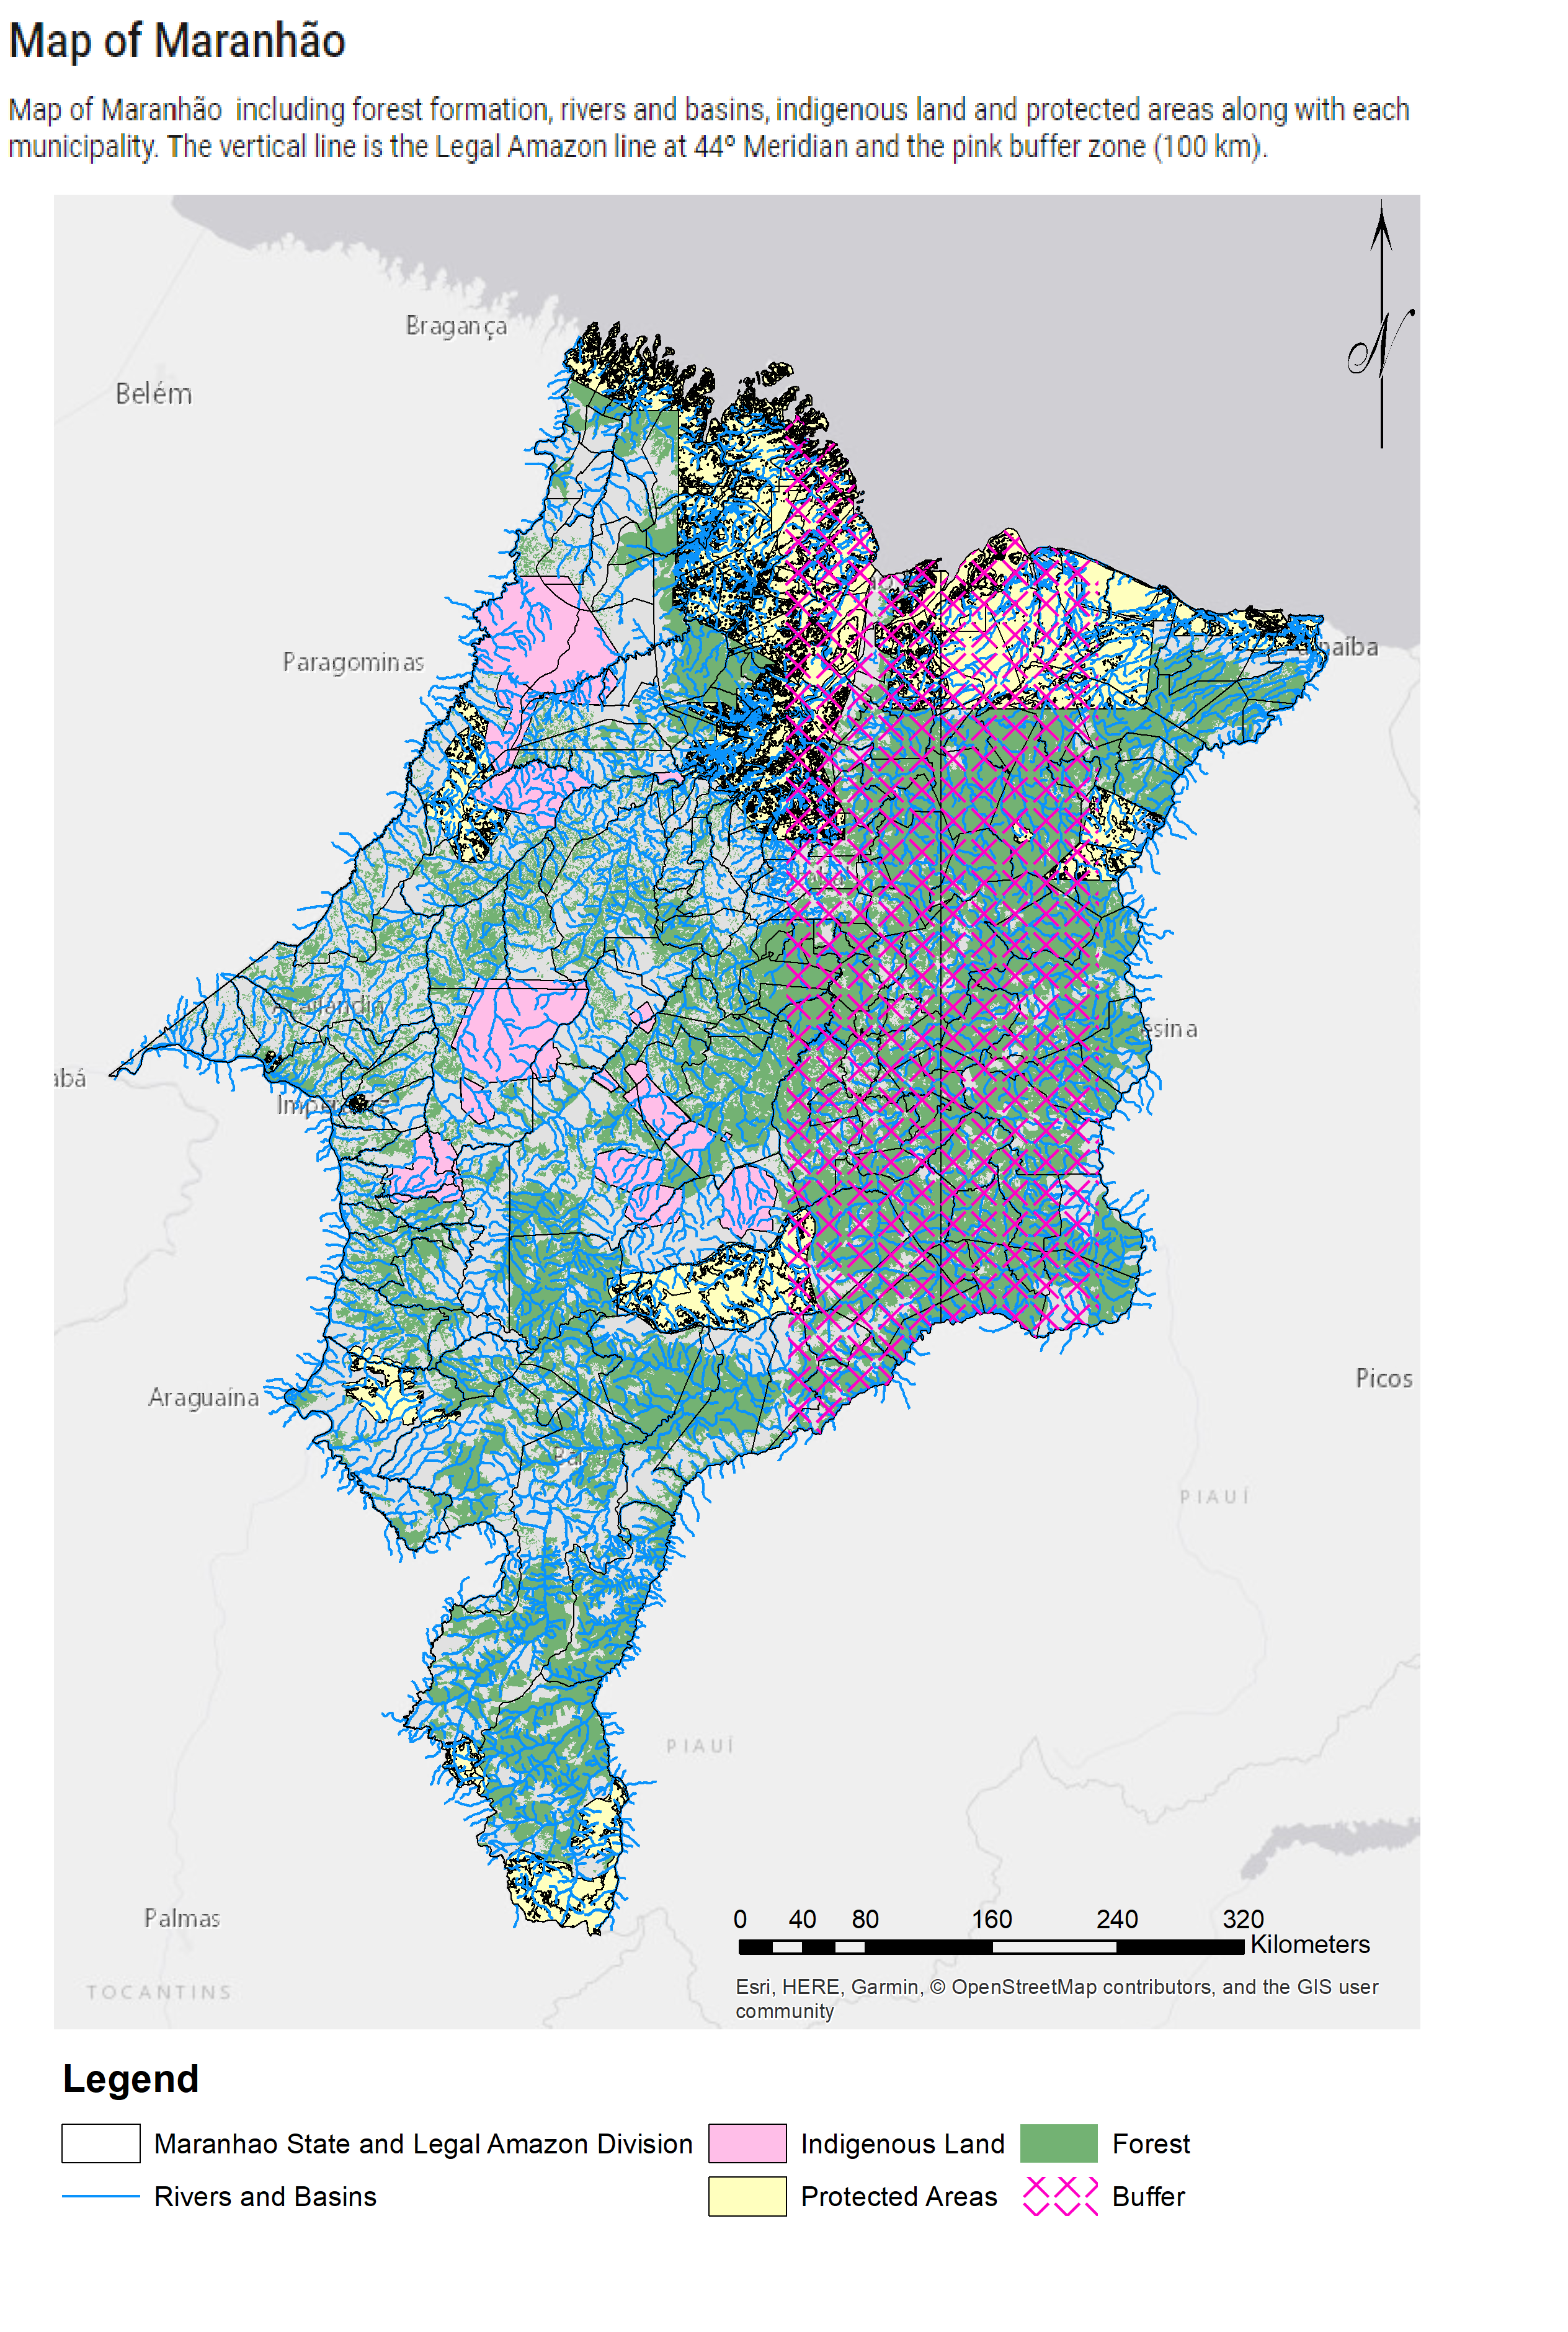
\includegraphics[width=1\textwidth, inner]{buffer_veg21.png}
\caption{Source: \citep{MMMAwebsite,nugeo_2018,embrapa_2018}.}
\label{fig:buffer}
\end{figure}

%In climatic terms, the region presents large oscillation from north to south, predominating the tropical climate of the equatorial zone. In the LM region, the hot and humid tropical climate (As) predominates, typical of the Amazon region. The eastern region is marked by warm and tropical wet-dry or savanna climate (Aw). Temperatures are high, with annual averages higher than 25ºC, and towards the southeast of the studied region, it reaches 28ºC.

%CITAR GRAHBER_2015.

%outras variaveis ambientais: chuva, temp,

 %The dry period, which occurs from July to November, with a lower incidence of rain around the month of August, registers averages of the order of 17.1mm. The average annual precipitation varies from 1,500 mm in the western portion (LM), reaching 1,800 mm near the coast, while in the MA area precipitation is lower with 1,700 mm peaks in the plateaus. There are even smaller records in the MA region, which can reach 1,000 mm. 

%  relevo

%The relief of Maranhão is characterised by low planing surfaces in the midst of extensive fluvial plains, much of it is enclosed by Paleozoic and Mesozoic rocks of the Parnaíba Sedimentary Basin. 

The Study area is characterised by the occurrence of a rainfall regime with two well defined seasons. The rainy season, which is concentrated from December to June, reaching the highest peaks of rain in the month of March. The sample region presents itself as a large sloping platform in the south-north direction, with a low dip to the Atlantic Ocean.  The relief is classified into two large units: plains, which are subdivided into smaller units, and plateaus. Plains are considered to be surfaces with dimensions of less than 200 meters. The plateaus are areas with heights above 200 meters, restricted to the south-central areas of the studied region \citep{feitosa_2006, bolfe_2013}. Information on the geology of the ecotonic region were extracted from the official map published in 2011 by the Brazilian Institute of Geography and Statistics (IBGE) on the scale 1: 1,400,000.


%Geologia 
%The Oxisols are predominant in Maranhão. They are consist of stable, highly weathered, tropical mineral soils with highly oxidized subsurface horizons. In spite of the low natural fertility, these soils present physical conditions favourable to the agricultural crop, mainly the mechanized, because they are deep soils, well drained and they normally occur in flat relief or gently mountainous.

% MATERIAL SOBRE EXPOSICAO SOLAR DO MARANHAO

Solar radiation on the terrestrial surface has direct implications for local meteorology, especially in the studies on climate variability, interfering in satellite image analysis \citep{cohen_2002, dasilva_2004, pereira_2017}. The study region here is privileged in its energetic potential, since it is located completely in the region bounded by the Tropics of Cancer and Capricorn, and close to the Equator, a condition that favors high rates of solar irradiation. The State of Maranhão presents an average annual global irradiation value of approximately 5.0 kWh / m2 \citep{pereira_2017}. In the ecological tension zone, i.e. studied area, the municipalities of Caxias (5.4 kWh / m2) (MA), Chapadinha (5.3 kWh / m2) (MA), Bacabal (4.9 kWh / m2)(LM) and São Luís (4.9 kWh / m2) (LM) are distinct for having the highest solar irradiation rates. 

%COLOCAR MAPA IGUAL AO DE GRAHBER_2015 LOGO APOS OS FATORES CLIMATICOS

%Aspectos vegetacionais: quais classificacoes vegetacionais? 

%Also in this region, the transitioning vegetation is characterised by the contact of Savana / ombrophilous forest (SO), Savana / Seasonal Forest (SN), and Savana / Seasonal Savana besides the presence of secondary vegetation within the domain \citep{bolfe_2013}.

%outras variaveis ambientais: hidrologia e hidrovia


\subsection{Data preparation}  %mudar o titutlo

%Paragrafo com softwares usados, packages e livros guiados

Handling and preparing spatial data requires specific softwares. I used ArcMap 10.4.1, ArcPy 10.4.1, and the extensions Geostatistical Analyst, Spatial Analyst and Spatial Statistics from ArcToolbox \citep{esri_2016,arcpy_2016}, and MATLAB R2017a and its Statistics and Machine Learning and Image Processing Toolbox \citep{matlab_2017}. For statistical analysis and modelling I worked with R \citep{R_2018} and several packages specially 'MASS'\citep{MASS_2002}, 'mgcv' \citep{Wood_2003, Wood_2004, Wood_2011, Wood_2017} and 'gratia' \citep{Gavin_2018}.

\subsubsection{Vegetation Indices} %PRECISO COLOCAR MAPA COM A LOCALIZACAO DA REGIAO DE ESTUDO TIPO AQUELE TILE DO MUNDO!!!!!! 
Two remotely sensed datasets were used – Vegetation Indices 16-Day L3 Global 250m MODIS13Q1 and Land Cover Type Yearly L3 Global 500m MODIS12Q1. These products were retrieved from the online Application for Extracting and Exploring Analysis Ready Samples (AppEEARS) tool courtesy of the NASA EOSDIS Land Processes Distributed Active Archive Center (LP DAAC), USGS/Earth Resources Observation and Science (EROS) Center, Sioux Falls, South Dakota, \citep{didan_2015,didan_munoz_2015,sulla_2015,sulla2_2018}.

In the AppEEARS tool it is possible to define the region of interest by uploading a polygon file in shapefile format and the output file format is in Georeferenced Tagged Image File Format (GeoTIFF). When selecting GeoTIFF, one GeoTIFF will be created for each feature in the input polygon file for each layer by observation. After defining the area of interest, the tool uploads the input polygon and reproject the input file to the source projection for each data product using the Geospatial Data Abstraction Library (GDAL) (‘gdalwarp’ function and the PROJ.4 definition) for each data collection \citep{usgs_2018}. In this manner the MODIS images from MODQ131 and MCD12Q1 products were acquired in GeoTIFF format and the projection chosen was the geographic datum WGS84 – EPSG:4326. Two shapefile with the same coordinate system were used to extract the location LM and MA. LM (Legal Maranhao) refers to the area under the surveillance program to the west of the Legal Amazon line and, the MA (Cerrado Maranhao) refers to the area comprising the east portion of the buffer zone (see Figure \ref{fig:buffer}).

Next, a bounding box for each feature in the MODIS file was determined using the minimum and maximum latitude and longitude values, with a one pixel buffer applied to each corner. For each feature, the tool determines which spatial tiles intersect with the bounding box, and the tiles are then extracted from OPeNDAP \citep{ cornillon_2003} and mosaiced into a single image. The process is repeated and the MODIS images are ultimately configured into a time series image stack for each feature in the file. Reprojection is performed using nearest neighbour resampling technique and the latitude and longitude of the sample region are maintained in the conversion. Nearest neighbour resampling was selected to ensure that categorical data sets including quality data layers are able to be transformed \citep{usgs_2018}. 

A total of 776 images of the Vegetation Indices product MOD13Q1 were downloaded, from February 2000 to December 2016, and 16 images of the product Land Cover MCD12Q1 for the years 2001 to 2016. Also from the product bands MOD13Q1 the composite band day of the year was obtained, which provides the date (day of the year: 1 to 366) of acquisition of each pixel that composes the image; the band pixel reliability summary quality assurance - QA, which provides a summary of the quality of the pixels; and VI Quality detailed - QA band, which provides detailed pixel quality information. The product bands MCD12Q1 was downloaded the Land Cover type quality check – QC along with five different types of land cover data set.

\subsubsection{Climatic variables} %PRECISO COLOCAR UMA TABELA COM A LOCALIZACAO LAT LONG DA ESTACAO , O NUMERO DA ESTACAO, ALTITUDE E SITUACAO  
%Paragrafo com explicacao da aquisicao dos dados INPE colocando de onde peguei e citando as fontes de cada dado pego


The climatic data were obtained from the Meteorological Database for Teaching and Research of the National Meteorological Institute (BDMEP – INMET in Portuguese), which stores historical series of several conventional meteorological stations of the INMET station network. The access is through registration but is freely available for academic purposes \citep{bdmep_2018}. Each conventional weather station (see Table \ref{estacoesconvecionais} for the 9 stations in the sample area is composed of several isolated sensors that continuously record the meteorological parameters (e.g., temperature, precipitation, humidity, and solar radiation), which are annotated by an observer that sends the measurements to a collection center. In the historical series the maximum temperature is taken at 00 Universal Time Coordinated (UTC) of the day and the minimum temperature is collected at 12 UTC of the day. Precipitation is calculated by accumulating the last 24 hours collected at 12 UTC and solar radiation equals the number of hours the sun shines directly onto the surface as long as it is not blocked by clouds or any other obstacles. The relative humidity is obtained by the readings of the wet bulb temperature and dry bulb temperature at 12.00, 18.00, and 24.00 UTC \citep{vianello_2011}. We use the monthly average maximum temperature (MAMxT), monthly average compensated temperature (MACT), monthly average minimum temperature (MAMT), monthly average precipitation (MAP), monthly average relative humidity (MARH) and number of hours of sunlight in a month as total solar radiation (TS) from February 2000 to December 2016. 

\begin{table}[H]
\footnotesize
\caption{INMET Metereological Stations}
\begin{tabularx}{\linewidth}{H H H H H H}
\hline
\hline
Station Number (ID)  & Latitude & Longitude & Altitude & Name & \centering\arraybackslash Area\\
\hline
82571	&	-5.5	&	-45.23	&	153	&	BARRA DO CORDA 	& LM		\\
82970	&	-9.5	&	-46.2	&	285	&	ALTO PARNAIBA 	& LM		\\
82460	&	-4.21	&	-44.76	&	25	&	BACABAL 	& LM		\\
82765	&	-7.33	&	-47.46	&	193	&	CAROLINA 	&	LM	\\
82376	&	-3.26	&	-45.65	&	45	&	ZE DOCA  &	LM	\\
82476	&	-4.86	&	-43.35	&	104	&	CAXIAS 	&	MA	\\
82382	&	-3.73	&	-43.35	&	104	&	CHAPADINHA 	& MA	\\
82676	&	-6.03	&	-44.25	&	180	&	COLINAS  &	MA	\\
82280	&	-2.53	&	-44.21	&	51	&	SAO LUIS &	MA	\\
\hline
\hline
\multicolumn{6}{l}{\footnotesize  Note: Source: \cite{bdmep_2018,inmet_2018}.}
\end{tabularx}
\label{estacoesconvecionais}
\end{table}

\subsubsection{Cross Validation} 

Cross validation is a necessary approach when dealing with remote sensing data. MODIS Vegetative Cover Conversion (MOD44A) was acquired from the Global Land Cover Facility - University of Maryland \citep{glcf_2018} to conduct a validation process regarding the response variables (NDVI and EVI). The VCC product is used as an indicator of change and not as a means to measure change. It is available for vegetation burning and anthropogenic deforestation types of land cover conversion. In this sense, using this product as an indicator of accuracy is useful and reliable as states \citet{defries_2002}.

As part of the validation process, we used a finer resolution data set to check the accuracy of the algorithm applied to the MOD13Q product. \citet{Hansen_2013} provided results from time-series analysis of Landsat images in characterising the global forest extent and change from 2000 through 2017. The scenes utilised for the analysis contained forest losses during the period 2000–2016, defined as a stand-replacement disturbance, or a change from a forest to non-forest state. Encoded as either 0 (no loss) or else a value in the range 1–16, representing loss detected primarily for the years 2001–2016 \citep{gfc_2017}.\footnote{Data Source: Hansen/UMD/Google/USGS/NASA. Data available on-line from: http://earthenginepartners.appspot.com/science-2013-global-forest.} Moreover, in 2018 Brazil's Spatial Research Institute (INPE), in accordance with the Brazil's Envinromental Ministry, published a data set covering the forest loss in the Cerrado Biome. This data consists of bi-annually images from 2000 to 2012 and yearly images from 2012 to 2016. Several sensors were used to create the composite data set, such as TM/Landsat5, ETM+/Landsat7, OLI/Landsat8, and LISS-III/IRS2. At a finer resolution, this product is a justified comparison between national and international land change products proving to be an acceptable validation procedure \citep{brito_2018}.


\subsection{Data Exploration and Interpretation}

After the selection of the variables there is a refinement process which configures the most important part of the research in order to achieve usable answers for statistical modelling. In this session, we will describes the steps taken to conduct the statistical analysis and the statistical method applied to the study.

\subsubsection{Response Variable}  %mudar o titutlo

% Paragrafo explicando como se deu a aquisicao dos pixels e tecnicas utilizadas interpretando por meio de figuras (colocar 2). 

In order to perform the analysis, NDVI and EVI images were imported onto MATLAB and scaled to the valid range of -0.2 to 1. Two images per month for each year were uploaded - excluding October and November during leap years because they had only one image within the month. The VI Quality detailed - QA band for each scene was converted to unsigned16bit according to the VI User Guide \citep{didan_munoz_2015} and it was used to create a Goodness mask to exclude pixels with clouds and not produced due to other reason than clouds. 

Before filtering the NDVI and EVI scenes with the VI mask, it was necessary to condition NDVI and EVI values to a specific threshold so to avoid values not related to forest. The criterion was taken following \citet{geerken_2009} and \citet{bayma_sano_2015} parameters to characterise forest in a transitional biome. Next, the VI indices are filtered and only values retained that have good quality according to the Goodness mask under the elimination of cloud coverage. 

With the Land Cover product MCD12Q1 it was required to resize and interpolate each image to the corresponding sizes of NDVI and EVI images. The interpolation method utilised followed a deterministic method called Nearest Neighbourhood (NN) or Thiessen method. The nearest method was considered because there is no extrapolation of the data, which would not have been suitable for categorical data and because it showed to be the fastest computation method with modest memory requirements \citep{ SLUITER_2009, matlab_2017}. After the interpolation, a land cover mask was produced to select only pixels in the images presenting forest classification. Following \citet{sulla2_2018}, the University of Maryland classification which corresponded to Land Cover Type 2 in the MCD12Q1 product was selected. The mask included different types of forests with at least 40\% of tree cover and canopy higher than 2m (see table \ref{UMD} detailing each class definition). Forests presenting less than 40\% of tree cover were excluded because this does not characterise a transitioning forest being predominantly assigned to Cerrado biome only \citep{bayma_sano_2015}.  

\begin{table}[H]
\footnotesize
\caption{University of Maryland (UMD) legend and class definitions}
\begin{tabularx}{\textwidth}{l c X}
\hline
\hline
Name & Class & \centering\arraybackslash Description\\
\hline
Water	&	0	&	At least 60\% of area is covered by permanent water bodies	\\
Evergreen Needleleaf forest	&	1	&	Needleleaf Forests 1 Dominated by evergreen conifer trees (canopy >2m). Tree cover >60\%.	\\
Evergreen Broadleaf forest	&	2	&	Dominated by evergreen broadleaf and palmate trees (canopy >2m). Tree cover >60\%.	\\
Deciduous Needleleaf forest	&	3	&	Dominated by deciduous needleleaf (larch) trees (canopy >2m). Tree cover >60\%.	\\
Deciduous Broadleaf forest	&	4	&	Dominated by deciduous broadleaf trees (canopy >2m). Tree cover >60\%.	\\
Mixed forest	&	5	&	Dominated by neither deciduous nor evergreen (40-60\% of each) tree type (canopy >2m). Tree cover >60\%.	\\
Closed shrublands	&	6	&	Dominated by woody perennials (1-2m height) >60\% cover.	\\
Open shrublands	&	7	&	 Dominated by woody perennials (1-2m height) 10-60\% cover.	\\
Woody savannas	&	8	&	Tree cover 30-60\% (canopy >2m).	\\
Savannas	&	9	&	Tree cover 10-30\% (canopy >2m).	\\
Grasslands	&	10	&	 Dominated by herbaceous annuals (<2m).	\\
Permanent Wetlands	&	11	&	Permanently inundated lands with 30-60\% water cover and >10\% vegetated cover.	\\
Croplands	&	12	&	At least 60\% of area is cultivated cropland.	\\
Urban and built-up	&	13	&	At least 30\% impervious surface area including building materials, asphalt, and vehicles.	\\
Cropland/Natural Vegetation Mosaics	&	14	&	Mosaics of small-scale cultivation 40-60\% with natural tree, shrub, or herbaceous vegetation	\\
Non-Vegetated Land	&	15	&	At least 60\% of area is non-vegetated barren (sand, rock, soil) or permanent snow and ice with less than 10\% vegetation.	\\
Unclassified	&	255	&	 Has not received a map label because of missing inputs	\\
\hline
\hline
\multicolumn{3}{l}{\footnotesize  Note: Source: \cite{sulla2_2018}.}
\end{tabularx}
\label{UMD}
\end{table}

Finally, to obtain a certain variation within each month, values of NDVI and EVI of the first period, with 15 first days of the month, were compared to the second period, with 30 days of the month. The assumption considered is explained in Table \ref{assumption}. In this sense, the final scene/image would present pixels assuming the highest quality and no cloud coverage. At the end of the process, pixels were selected within the bandwidths of 100km, 50km, and 25km - measured departing from the artificial Legal Amazon line to the west and east portion of the State. When the pixel had a variation greater than 0.1 within a month, it was considered a disturbance.

\begin{table}[H]
\footnotesize
\caption{Algorithm Assumption}
\begin{tabularx}{\linewidth}{X X X}
\hline
\hline
$NDVI_{1} > NDVI_{2}$	& ->  $NDVI_{1} - NDVI_{2}$	 & Numbers (1) and (2) refer to the order of the period of the month \\
$NDVI_{1} <= NDVI_{2}$	& ->  $NDVI_{1} = NDVI_{2}$	 & Numbers (1) and (2) refer to the order of the period of the month. The second equation assumes that values did not change within the month and then the value assigned is from the last observation	\\
\hline
$EVI_{1} > EVI_{2}$	& ->  $EVI_{1} - EVI_{2}$	 & Numbers (1) and (2) refer to the order of the period of the month \\
$EVI_{1} <= EVI_{2}$	& ->  $EVI_{1} = EVI_{2}$	 & Numbers (1) and (2) refer to the order of the period of the month. The second equation assumes that values did not change within the month and then the value assigned is from the last observation 	\\
\hline
\hline
\end{tabularx}
\label{assumption}
\end{table}


The approach above was undertaken for all the images corresponding to NDVI and EVI values for each month of each year, giving 406 final image results. For the leap year, the process stopped at the land cover mask filtering process. To compose a panel for each monthly period over 17 years, we took the sum of pixels signalled as disturbed for each of 406 images. 

\subsubsection{Covariates Variables} \label{covariate variables}  %mudar o titutlo

The climatic variables needed a more complex processing system since the data from weather stations were sparse. First, all the data was in a tabular format, i.e. all variables in one table, and geographic locations in the form of latitude and longitude coordinates and z-coordinates, such as elevation values, was created for each weather station using ArcMap. After localising the x,y,z coordinates, a shapefile for each station was created. Then the shapefiles were selected and extracted by year, using ArcPy environment. 

Next, an interpolation method was used to deal with areas with no data available. The method chosen was ordinary (point) Kriging which has been argued as the best interpolation technique available for sparse data \citep{SLUITER_2009}. Ordinary kriging is part of the probabilistic methods in which the concept of randomness is incorporated into the analysis. This method is the basic form of Kriging, where the prediction relies on a linear combination of the measured values and the spatial correlation between the data, determining the weights. As the mean is unknown we assume that intrinsic stationary exists in the data. This assumption may fail for our data set since this type of data are usually not stationary. To overcome this issue we used different sizes and shapes of neighbourhood to adjust the kringing ordinary model \citep{SLUITER_2009}. 

After the interpolation, the images were converted to raster, resampled to the size of the response variable, and exported to MATLAB environment. Generally, for temperature, precipitation, and other climate data, the best way to interpret and study these phenomenons is using anomaly measurements which corresponds to the difference between measurement and mean. In this sense, the average value of the variable of each image for each month and each year was computed, giving a total of 408 images analysed for both regions (MA and LM), and for each climatic variable, a total of 2,448 images. Following this procedure, the number of pixels with values higher and lower than the average value of the variable was extracted to a table. At the end, the table contained above and below values compared to the mean for each variable translating into 12 variables.

A summary TABLE OR GRAPH of the response and explanatory variables of this study is presented at TABLE GRAPH XXX.

\subsubsection{Modelling deforestation trends}  %mudar o titutlo

%Descrever modelos passados de desmatamento

Many recent studies of land cover changes focus explicitly on taking account of the trends and changes in the rates of environmental transformation in terms of their driving forces. More precisely, these studies try to identify the major causes of land-cover change within different geographical and historical contexts \citep{GEIST}. To this end proximate and underlying causes of deforestation models are concerned by the fact that some causes are direct in the sense that their occurrence or variation generates more or less deforestation through simple channels, while other causes are indirect in that they impact on the sources of deforestation through more complex channels \citep{MOTEL}. In this regard, the physical environment strongly influences where agents deforest, where many studies provide evidence that forests in drier, flatter, higher-fertility areas, with adequate drainage and thus more suitable for agriculture are more likely to be cleared \citep{ANGELSEN4}. In contrast, poor soil quality is also reported to lead to relatively high deforestation, since scant soil endowment fuels accelerated clearing for other activities, such as pasture \citep{GEIST,COSTA}. 

Environmental factors and  biophysical drivers are also increasingly being recognised as not only playing a role but being fundamental in deforestation \citep{GEIST}. To cite, \citet{BARNI} showed that, independent of the rate and magnitude of deforested areas, the areas affected by forest fires were dependent on the forest type and climate factors. Zones with ecotone influence tended to be deforested more than zones without ecotone influence, i.e., the more dense a forest is the less deforested will be. In addition, the largest occurrence of forest fires was observed in the zones with ecotone influence in years with \textit{El Nino} events, such as Maranhao state. The analysis also indicated that the areas most affected by forest fires during the studied period were associated with strong climatic events and the occurrence of these fires was amplified in the zones with ecotone influence \citep{BARNI}. These facts strongly suggest that it is pertinent to control for climatic aspects in ecotone zones when studying trends in deforestation.\footnote{In this study, ecological tension zone, ecotone zones and transitional forest have the same meaning. } 



%According to \citet*{MOTEL}, there are at least four models to study the impact of deforestation and its trends. 

%The first model included variables related to governance and institutional improvements as flatters for reduce the level of deforestation. The Environmental Kuznets Curve (EKC) model generally view better governance as an efficient means to achieve lower deforestation rates or environmental degradation while pursuing economic development. 

%Considering studies that describe the \textit{ex-ante} and \textit{ex-post} deforestation occurrence, the second model takes into account reforestation activities, which corresponds to the phenomenon occurring in many developed countries. Rather than considering overall deforestation, \citet*{MOTEL} explained that a model of Compensated Successful Efforts (CSE) would be appropriate to developing countries in order to fulfil the requirements established by the Reduced Emissions from Deforestation and Degradation mechanism. 



%In this context, many studies \citep{FENGER,DONG,LAMBIN1,FARGIONE,BARONA,ALDRICH,RICHARDS,KEENEY} concentrates in understanding causes of deforestation and land use changes to curb deforestation. In these studies, most commonly, a combination of proximate and underlying causes have been identified as the main drivers of deforestation.

\textbf{Statistical Modelling} 

%The most common approach used to model deforestation would be a linear model with a single or multiple terms. However, things are rarely this simple, and the model might interact in a complex way. The four approaches presented earlier consider the linear model as the first premise of the analysis but they are challenging when dealing with non-linear relationship found between variables \citep{griffin_2012}. In environmental analysis the data are seldom modelled adequately by linear regression models. 


%Introduzir o conceito de GAM 

For most ecological and climatic data sets at least some of the assumptions underlying a linear regression model are unlikely to be valid \citep{zuur_2011}.   To address this issue we here employ a generalized additive model (GAM). A literature review shows that GAMs are not extensively applied to deforestation models. \citet{COHEN_2008} showed that social factors appear to play a critical role that may ultimately determine disease risk when evaluated with environmental and climatic factors. They modelled incidence rates of a disease in Cuba as the response variable and deforestation as one of the exploratory variables. \citet{MENDES_2012} observed the relationship of deforestation, corruption and economic growth in the region of Legal Amazon, in Brazil and found no statistical evidence for the existence of a Kuznets curve. \citet{GREEN_2013} used a binomial GAM model to account for forest and habitat losses in protected areas on the Eastern Arc Mountains of Tanzania. More recently, \citet{BEBBER_2017} studied the impact of protected areas on global carbon emissions in America, Africa and Asia. They used splines regressions in GAMs and suggested that tropical PAs overall reduced deforestation carbon emissions by 4.88 Pg, or around 29\%, between 2000 and 2012. 


A GAM is a generalized linear model with a linear predictor involving a sum of smooth functions of covariates. Mathematically, GAM is an additive modelling technique where the impact of the predicted variables is captured through smooth functions \citep{larsen_2015}. In general, the model has a structure defined as: 

%\begin{center}
\begin{equation}  \label{eq:3} 
g(\mu_{i}) = A_{i} \theta + f_{1}(x_{1i}) + f_{2}(x_{2i}) + f_{3}(x_{3i},x_{4i}) + \dots
\end{equation}
%\end{center}

where $\mu{i} \equiv \displaystyle \E(Y_{i})$ and $Y_{i} \sim EF(\mu_{i},\phi)$. $Y_{i}$ is a response variable, $EF(\mu_{i},\phi)$ denotes an exponential family distribution with mean $\mu{i}$ and scale parameter, $\phi$, $ A_{i}$ is a row of the model matrix for any strictly parametric model components, $\theta$ is the corresponding parameter vector, the $f_{j}$ are smooth functions of the covariates, $x_{k}$, and ${i}$ refers to the unit of analysis \citep{Wood_2017}. This model allows for flexible specification of the dependence of the response on the covariates because the smooth functions are nonparametric. The smooth function $f_{j}$ is represented by basis expansions for each smooth, each with an associated penalty function controlling  smoothness. According to \citet{Wood_2004, Wood_2017}, the estimation can be carried out by penalised regression methods, and the appropriate degree of smoothness for $f_{j}$ can be estimated from data using cross validation or marginal likelihood maximisation.

The smooth function $f$ is composed of the sum of basis functions b and their corresponding regression coefficients $\beta$, written in the form of:

%\begin{center}
\begin{equation}  \label{eq:4} 
f(x) = \sum\limits_{j=1}^k b_{j}(x) \beta_{j}, \\
\end{equation}
%\end{center}

where k is the basis dimension (\citet{Wood_2017}, p.162). 

%In this way, it is possible to estimate $f$ in such a way that becomes a linear model. The smooth functions are also called splines or penalised splines. Splines are real functions that are defined by multiple sub-functions, where the polynomial pieces connect are called knots. The family of splines includes cubic splines, which fits a third-order polynomial on parts of the data and ensures that at the knots, the connections are smooth \citep{zuur_saveliev_ieno_2014}. It is important to observe that at the ends of the data, there will be discontinuity in the value taken by the spline. When the variable of interest behaves cyclically, it is necessary a correction procedure to these splines. The cyclic cubic spline is a potential solution to the problem because its basis has an additional constraint, which forces to no discontinuity at the end points of the spline \citep{Gavin_2018}.


%The choice of degree of model smoothness is essentially arbitrary and finding the optimal number of knots for a regression is obtained by finding the parameters $\beta$ and the smoothers that minimise the criteria in equation \ref{eq:5} \citep{zuur_saveliev_ieno_2014}.

%\begin{center}
%\begin{equation}  \label{eq:5} 
%\| Y - X\beta \|^{2} + \lambda \int_{}^{} f '' (x)^{2}dx\\
%\end{equation}
%\end{center}

%The second part of equation \ref{eq:5} is a penalty and contains $\lambda$ and an integral over the second-order derivatives, telling how smooth a curve is. A high value of $f''$ means that the smoother f is highly non-linear whereas a straight line has a second derivative equal to 0. In this case, if $\lambda$ is very large, the penalty for having a non-smooth curve is also large and if $\lambda$ is small, then there is a low penalty for non-smoothness \citep{zuur_saveliev_ieno_2014}. 

%In other words, when $f$ is very wiggly the penalty will take high values and when $f$ is ‘smooth’ the penalty will be low. If $f$ is a straight line then the penalty is actually zero. So the penalty has a null space of functions that are un-penalised: the straight lines in this case. Choosing the value of $\lambda$ requires further techniques. If $\lambda$ is too high or too low  then the data will be over-smoothed or under-smoothed, in both cases this will mean that the estimate $f$ will not be close to the true function $f$. Ideally, it would be good to choose $\lambda$ so that $f$ is as close as possible to $f$ \citep{Wood_2017}. A possible solution might be to choosing  $\lambda$ to minimise $\mathit{V_{o}}$ known as the ordinary cross validation using $\hat{f}$ estimation to fit all the data

%\begin{center}
%\begin{equation}  \label{eq:6} 
%\mathit{V_{o}} = \frac{1}{n} \sum_{i=1}^{n}\frac{(y - \hat{f_{i}})^{2}}{(1 - A_{ii})^{2}}\\
%\end{equation}
%\end{center}

%where \textbf{A} is the corresponding influence matrix, which is just the influence matrix for the model fitted to all the data. In practice, the $A_{ii}$ is replaced by their mean, resulting in the generalized cross validation score (GCV) \citep{Wood_2017}

%\begin{center}
%\begin{equation}  \label{eq:7} 
%\mathit{V_{g}} = \frac{n \sum_{i=1}^{n}(y_{i} - \hat{f_{i}})^{2}}{{[n - tr (\textbf{A})]^{2}}}\\
%\end{equation}
%\end{center}

%Interpretability 

%Flexibility and Automation

%Regularization

It is possible to regularise the smoothness of the predictor functions to prevent overfitting using the generalized cross validation score. Technically, GAM is an additive modelling technique where the impact of the predictive variables is captured through smooth functions, but provides a regularised, automatic and interpretable solution. Considering an additive model, the interpretation of the marginal effects of a single variable does not depend on the values of the other variables in the model. Also, predictor functions are automatically derived during model estimation \citep{larsen_2015}. 


%Dar exemplos de contribuicao desta metodologia para o desmatamento e em especial desmatamento na floresta tropical, amazonia e cerrado (floresta de transicao).



\textbf{Autocorrelation} %mudar o titutlo

In principle, when the nature of the data is time series, the timing of one period may depend on the timing of the previous year. This means that one should check for the possibility of autocorrelation and if necessary take into account of such the auto-correlation in the data. In GAMs it is possible to include an ARMA error structure. More precisely, the ARMA model has two parameters defining its order with the number of auto-regressive parameters (p) and the number of moving average parameters (q). Model \ref{eq:3} now can be expressed as


%\begin{center}
\begin{equation}  \label{eq:8} 
g(\mu_{i}) = A_{i} \theta + f_{1}(x_{1i}) + f_{2}(x_{2i}) + f_{3}(x_{3i},x_{4i}) + \dots + \varepsilon_{i}
\end{equation}
%\end{center}

where $\varepsilon_{i} = {\phi}\varepsilon_{i-1} + {\phi}\varepsilon_{i-p} + \eta_{i} $ is modelled as a function of the residuals of the p previous time points and white noise, and $\varepsilon_{i} = {\theta}\eta_{i-1} + {\theta}\eta_{i-q} + \eta_{i}$ is modelled as a function of the disturbance term and a past value of this disturbance term \citep{zuur_saveliev_ieno_2014}.

\textbf{Quantifying deforestation} 

The generalized additive model (GAM) with an exponential family distribution has been the most widely applied method to measure and quantify the non-linear association between phenology and covariates, such as meteorological conditions, mainly because it allows for non-parametric adjustments of non-linear confounding effects of seasonality and trends; \citep{alkemad_1998,BELL_2015,JOYE_2015,LUSK_2016,SADAT_2016,HALPERIN_2016, SANTOS_2017,TAPIA_2017,LIU_2018,MORENO_2018}.  In an attempt to quantify forest disturbance as proxy for deforestation, we apply a GAM with a negative binomial distribution and a logarithmic link function. The negative binomial distribution suitable for this study since the variance of deforestation is much larger than the mean, which is frequent feature of ecological data \citep{zuur_2011}. More precisely, the means of NDVI and EVI are to 0.04\% and 0.01\% of their variance, respectively. Hence, the response variable is negative binomial distributed. The full description is as follows:

\begin{flushleft}
 \hspace{4em} $Y_{is}$ $\sim$ NB($\mu{_i}$,k) 
\vspace{-0.2em}
\begin{equation}
\hspace{-12em}E(Y_{i}) = \mu_{i}, and \hspace{1em} var(Y_{i}) = \mu_{i} +\frac{\mu^{2}_{i}}{k} \label{eq:9}    
\vspace{-1em}
\end{equation}
 \hspace{4em} log($\mu_{i}$) = $\alpha$ + $f_{j}$($X_{i1})$ $+ \dots +$ $f_{j}(X_{iq})$ \hspace{1em} or  \hspace{1em} $\mu{i}$ = $e^{\alpha +f_{j}(X_{i1})+\dots+f_{j}(X_{iq})}$  \\    
\end{flushleft}

$Y_{i}$ is the response variable at observation i. The notation $f_{j}$($X_{i1}$) stands for 'smoothing function of the covariate variable X', and \textit{NB} is a negative binomial distribution with mean $\mu_{i}$ and dispersion parameter k. In general, negative binomial distributions are used to model overdispersed count data or Poisson data.  

The geometric distribution is a negative binomial with overdispersion parameter, k, set to 1. In this sense, the variance increases as a quadratic function of the mean \citep{zuur_saveliev_ieno_2014}. Correcting the data for overdispersion with the geometric distribution, the model is stated as

\begin{flushleft}
 \hspace{4em} $Def_{\scriptscriptstyle (NDVI_{i}, EVI_{i})} = \alpha + f_{\scriptscriptstyle Year}(Year) + f_{\scriptscriptstyle Precip}(aPrecipitation) + f_{\scriptscriptstyle Max Temp}(aMax Temperature)$ 
\vspace{-0.2em}
\begin{equation}
  + f_{\scriptscriptstyle Min Temp}(bMin Temperature) +  f_{\scriptscriptstyle Sunlight}(bSunlight) + f_{\scriptscriptstyle Humidity}(bHumidity) \label{eq:10}    
\vspace{-1em}
\end{equation}
\end{flushleft}

%Colocar o modelo de desmatamento escolhido explicar cada variavel do modelo, novamente. 

where $Def_{\scriptscriptstyle (NDVI_{i}, EVI_{i})}$ is the response variable that can assume NDVI and EVI values for three different bandwidths (25km, 50km, 100km) in each month \textit{i}, and $i=1,\dots,204.$ The remaining variables are the intercept $\alpha$ andthe additive smoothing functions of the explanatory variables Year,  and the covariates Precipitation, Humidity, Max and Min temperature and sunlight. \textit{a} and \textit{b} refers to the sum of pixels above and below the mean, respectively.

%Explicar processo de escolha do modelo de desmatamento (forwarding selection, Zuur). 

The model selection followed the forwarding approach of \citealp[p.391]{zuur_saveliev_ieno_2014}. The model started with a GAM that used one variable, then fitted 13 different models and a different set of smoothers (penalised splines "ps", cubic splines "cr", and cyclic splines "cc") and compared their Akaike information criterion (AIC). The model with the lowest AIC was elected as the main model and, then it was fitted to 12 different models, each with the addition of the variable with the lowest AIC. The forward selection stopped at the moment the main model had the best AIC value comparing to the remaining models. After the model selection, an autocorrelation test was conducted but none of the models appeared to be autocorrelated. The model, including the splines takes the form of:

\begin{flushleft}
 \hspace{1em} $Def_{\scriptscriptstyle (NDVI_{i}, EVI_{i})} = \alpha + f_{\scriptscriptstyle Year}(Year, bs= cc) + f_{\scriptscriptstyle Precip}(aPrecipitation, bs= cr) +$ 
%\vspace{-0.2em}
\begin{equation}
 f_{\scriptscriptstyle Max Temp}(aMax Temperature, bs= cr) + f_{\scriptscriptstyle Min Temp}(bMin Temperature, bs= cc) +  \label{eq:11}    
%\vspace{-1em}
\end{equation}
 \hspace{1em} $f_{\scriptscriptstyle Sunlight}(bSunlight, bs=cc) + f_{\scriptscriptstyle Humidity}(bHumidity, bs= ps)$
\end{flushleft}


Due to the fact that his method is relatively recent, it is important to acknowledge that the algorithms available for choosing the optimal smoothing parameter are  not  yet  well  developed  and  can  generate  misleading  results if care is not taken. Furthermore,  use  of  such  criteria  can  often  lead  to  over-fitting  and  deliver  implausible  associations.  The choice  of  smoothing  parameters  for  smoothing  splines  in  GAM  should  therefore  always  be  accompanied  by  a  graphical  verification  of  functional  associations  with  the outcome  to  verify  clinical  plausibility \citep{moore_2011}.

\subsubsection{Model Validation}  %mudar o titutlo

Validating the results from the algorithm applied to the MOD13Q1 and MCD12Q1 images required features of the machine learning domain. In summary, machine learning algorithms can figure out how to perform important tasks by generalizing from examples. This is often feasible and cost-effective where manual programming is not \citep{Domingos_2012}.

There are different types of machine learning algorithms, where the most mature and widely used one is classification. According to \citet{Domingos_2012}, a classifier is a system that inputs a vector of discrete and/or continuous feature values and outputs a single discrete value, the class. For this study, the filter classifies pixels into deforested or not deforested and its input may be a Boolean vector $x = (x_{1},\dots, x_{j},\dots, x_{d})$ where $x_{j} = 1$ if the \textit{j}th pixel is deforested and $x_{j} = 0$ otherwise. A learner inputs a training set $(x_{i}, y_{i})$, where $x_{i} = (x_{i,1},\dots, x_{i,d})$ is an observed input and $y_{i}$ is the corresponding output, and output is a classifier. The test of the learner is whether this classifier produces the correct output $y_{t}$ for future examples $x_{t}$. A feasible classification validation is the confusion matrix. 

%Explicar aqui o metodo usado para fazer a confusion matrix.

The confusion matrix is a two by two table that contains four outcomes produced by a binary classifier. The classification scheme divides the data randomly into a training set, a test set and a validation set. The training method is the Scaled Conjugate Gradient (SCG), which is a supervised learning algorithm for feed-forward neural networks \citep{mor_1993}. In order to optimise the performance, an iterative random sampling approach is applied. The Cross-Entropy approach is based on sampling and updating an underlying distribution function over the set of feasible solutions \citep{HU_2009}. Finally, calculations for the confusion matrix are done based on minimum excluded (MEX) calculations \citep{matlab_2017}.

The four outcomes produced by the confusion matrix are true positive, true negative, false positive, and false negative. The true positives (TP) refer to the number of positives divided by all the positive outcomes and the same applies to true negatives (TN). False positives (FP) indicate the number of pixels assigned as positive but are, in fact, negative, divided by all the positive outcome. In turn, false negatives (FN) follow the same interpretation as false positives. 


%Explicar os metodos de validacao para as variaveis Response


To validate the response variable results, it was used the MODIS Vegetative Cover Conversion (VCC) for the available period (2000-2005). The product is further divided in Deforestation product (MOD44A${\_}$C) and Burn product (MOD44A$\_$B) and both were used to compute the validation test. 

The method for the deforestation product is derived from the original space partitioning method \citep{zhan_2002} and relies on a decision tree classification algorithm \citep{breiman_1984} to determine antecedent vegetation condition and compares this to current vegetation condition. Change due to burning product is derived using the difference Normalized Burn Ratio (dNBR) methodology from two scenes a year apart, as proposed by \citet{key_2004}.  Tests were computed per season (raining season and dry season) and per vegetation index (NDVI and EVI). The confusion matrix showed 100\% true positives and true negatives, which gives high stability to the algorithm created and applied to the NDVI and EVI indices. 

%ROBUSTNESS CHECK AND VALIDATION WITH HANSEN AND PRODES

Checking the results with other datasets was an alternative approach taken in this study. A confusion matrix was applied to the \citet{Hansen_2013} and Brazilian (INPE) data sets \citep{brito_2018}. The results showed no difference from the results presented in the VCC validation method. The confusion matrices are provided in the Appendix \ref{appendix}. 

%Explicar os metodos de validacao para as variaveis Explicativas 
The covariates variables were validated using cross-validation processes during the interpolation procedure. Cross-validation uses all the data to estimate the trend and autocorrelation models. It removes each data location one at a time and predicts the associated data value. This is also known as leaving-one-out, and can be computed for all or a subset of the data locations \citep{esri_2016}.

In the kriging method, the cross-validation produced other results that helped evaluate the best interpolation method. More specifically, the Average Standard Errors (ASE) and Root Mean Square Standardized Error (RMSE) were computed. If ASE from the model are close to the RMSE then the model is correctly assessing the variability in prediction. If ASE are greater than RMSE then the model is overestimating the variability of the prediction and, finally, if the ASE are less than RMSE, the model is underestimating the variability in predictions. For the covariates analyses, ASE were on average 95\% of the value of the RMSE, proving to be a reasonable interpolation method with valid results.

In terms of statistics, model validation with additive modelling was visual rather than numeric after the model selection phase. The steps taken included plotting the residuals against fitted values to identify violation of homogeneity, and plotting the residuals against each variable in the model and check for patterns. Also, a histogram of the residuals was examined to verify normality. 

%Criar um diagrama parecido com o de Griffin, p. 34 para descrever MODEL VALIDATION


\section{Results}  %mudar o titutlo

\subsection{Deforestation trend in a ecotone zone of Maranhao} \label{resultssection1}

%Explicar response over year

Our baseline model includes 204 monthly observations of NDVI and EVI values changing over the years with five influencing covariates (Precipitation, Max Temperature, Min Temperature, Sunlight and Humidity). The baseline model was applied to three different distance spans (25km, 50km, 100km) considering the Legal Amazon line.\footnote{It is important to acknowledge that the numerical results of the model should not be interpreted in the same manner as the linear regression results. According to \citet{Wood_2011} in \citet{zuur_saveliev_ieno_2014}, p-values close to 0.05 can be around half of their correct value when the null hypothesis is true. This means that smoothers with p-values smaller than 0.001 can be trusted but p-values of 0.02 to 0.05 need to be viewed with caution.} 

In general, the deviance explains the models close to the artificial line better. At large distances (100 km), most of the covariates do not have a significant effect, and thus will be omitted from this part of analysis. Table \ref{results1} gives the summary of the results including deviance, AIC, p-value, degrees of freedom, and the estimated value of the function. The best way to understand and interpret GAMs is through visual representation. Considering that the results produced several models, we define the name of these models according to the location status, whether in Cerrado Maranhao (MA) or Legal Maranhao (LM), the bandwidth or distance from the Legal Amazon line, in which are 25km,50km and, 100km, and, finally, regarding each response variable that in our case is related to NDVI (n) and EVI (e) values. We add an indicative variable to indicate raining (r) and dry (d) seasonality. Plotting the smoothing functions, it is possible to check for the path of deforestation through the years and the climatic state during that period. The blue line refers to positive changes in deforestation or increments, and the red line indicates negative changes in deforestation or decreases \citep{Gavin_2018}. 

\begin{table}[H]
\footnotesize
\caption{Models Output}
\begin{tabularx}{0.9\linewidth}{lxx}
\hline
\hline
Model  & AIC &   Deviance Explained\\
\hline
Baseline Model & & \\
\hline
ma25n & 4592.974 & 15\%\\
lm25n & 4753.342 & 30.9\%\\
ma25e & 5382.682 & 20.1\%\\
lm25e & 5450.606 & 36.4\%\\
ma50n & 5035.296 & 17.3\%\\
lm50n & 5010.875 & 24.5\%\\
ma50e & 6123.032 & 20.5\%\\
lm50e & 5921.597 & 29.3\% \\
ma100n & 5312.836 & 16.6\%\\
lm100n & 5318.571 & 30.5\%\\
ma100e & 6097.770 & 23.6\%\\
lm100e & 5901.040 & 33.4\%\\
\hline
Raining Season &    &\\
\hline
ma25nr & 3008.928 & 53.8\% \\
lm25nr & 3082.583 & 44\% \\
ma25er & 3486.908 & 52.1\% \\
lm25er & 3369.937 & 63.1\%\\
ma50nr & 3402.803 & 60\%\\
lm50nr & 3241.013 & 55.8\% \\
ma50er & 4154.889 & 62.6\%\\
lm50er & 3886.190 & 63.2\%\\
ma100nr & 3723.872 & 62.2\%\\
lm100nr & 3552.311 & 52.7\% \\
ma100er & 4176.352 & 59.4\% \\
lm100er & 3906.004 & 59.5\% \\
\hline
Dry Season&    &\\
\hline
ma25nd & 3029.610 & 52.3\% \\
lm25nd & 3330.420 & 54.6\% \\
ma25ed & 3533.256 & 50.9\%\\
lm25ed & 3812.126 & 65.6\%\\
ma50nd & 3390.411 & 42.2\%\\
lm50nd & 3498.748 & 35.1\%\\
ma50ed & 4051.907 & 47\%\\
lm50ed & 4112.314 & 48.5\%\\
ma100nd & 3562.066 & 45.2\%\\
lm100nd & 3701.532 & 47.2\%\\
ma100ed & 4051.806 & 45.3\% \\
lm100ed & 4097.055 & 46.7\% \\
\hline
\hline
\end{tabularx}
\label{results1}
\end{table}


With respect to the model \textit{ma25n}, the explained deviance is 15\%, the variance was set to 1 in the geometric negative binomial distribution. The explanatory variable year is significant at 1\% level, and the smoothers significant at 1\% level are \textit{Min Temperature}, \textit{Max Temperature}, \textit{Humidity} and \textit{Sunlight}. The degrees of freedom for the smoothers are 2.4, 6.8, 4 and 7.9. In summary, for MA at 25km, deforestation had a positive effect after 2010 and, through the years, deforestation decreased during periods of low humidity (high thermal oscillation). It is also deduced from the model that deforestation decreased during periods of more hours of sunlight. There were more deforested pixels in periods where temperature declined. 

For the model \textit{lm25n}, the explained deviance is 30.9\%, the explanatory variable year is significant at 5\% level, the smoothers significant at 1\% level are \textit{Max Temperature}, \textit{Humidity} and \textit{Sunlight}. The degrees of freedom for these smoothers are 8.6, 6.1 and 1.4. The results are similar to the \textit{ma25n} model by showing that deforestation also decreased during periods of less humidity and extreme higher levels of precipitation. Examining deforestation as a function of the year showed that there was a positive effect, i.e., increments on forest loss, during the beginning of the 2000's.

%Explicar o de \textit{ma25e} e o ml25e


Models with EVI values were considered better in terms of cross validation. Model \textit{ma25e} shows that deforestation increased over time with a positive peak after 2010. Deforestation also increased when the covariates sunlight and minimum temperature decreased. For maximum temperature, the negative effect is greater than the positive effect but, in essence, deforestation decreased with higher temperatures. On the Legal Maranhao side, the results of the model \textit{lm25e} show that all variables are significant at the 1\% level. The model explains 36\% of the changes in EVI values, i.e., deforestation. From 2007 to 2012, deforestation increased in the region. The positive effect happened during periods of higher temperature and low humidity. 


%explicar o de \textit{ma50n} e \textit{lm50n}
%Expanding the buffer zone to 50km, the model \textit{ma50n} shows the same pattern as 25km analysis with the difference that deforestation increased with higher levels of precipitation. The model explains 17.3\% of NDVI values for that region. Deforestation through the years had only a negative effect between 2002 and 2004 and the most of deforestation occurred when levels of sunlight were low. For the \textit{lm50n} model, it is also observed the same pattern with the exception that, at 50km band, deforestation declined with higher levels of temperature although the pattern for deforestation continued to decrease at extreme higher levels of precipitation. 

%explicar o de \textit{ma50e} e \textit{lm50e}

%Checking for EVI values, the model \textit{ma50e} still showed forest loss increment for the period after 2010, giving the same result as \textit{ma25e}. In turn, deforestation happened during low temperature period and with less hours of sun. It shows that at 50km, increased deforestation happened when precipitation level was higher than the average and deforestation and humidity had a negative linear relationship. This result differs from the \textit{lm50e} model, in this model, humidity and deforestation have a non-linear relationship and the latter occurred when the former was at low levels. Forest loss also happened when temperatures increased and, looking in function of the years, deforestation decreased after 2004 and increased back again after 2010. 


%explicar o \textit{ma100n} e \textit{lm100n} 

%For the last set of models with the largest bandwidth the deviance explained between 16\% to 33\% of deforestation in those areas. Starting by the model \textit{ma100n}, many of the covariates have lost significance. The explanatory variable year has no longer an effect on deforestation and higher levels of temperature have a linear negative relationship with deforestation. At the end, deforestation decreased during lower levels of humidity or, higher thermal oscillation. Model \textit{lm100n} showed that deforestation increased at higher levels of precipitation but when the levels of precipitation reached values higher than 75\% of the sample, deforestation decreased significantly. At 100km buffer, deforestation decreased during periods with less glaring sunlight.

%explicar o \textit{ma100e} e ml100e
%With the model \textit{ma100e}, deforestation increased during 2008 to 2012 with a slightly decrease in 2010. Deforestation varied considerable with the decay of humidity levels, this can also be mirrored with the temperature covariates, both seem to show that deforestation increased within their extreme values. Again, deforestation decreased with the increasing amount of precipitation during the studied period. Finally, the 100km band analysis for the Legal Maranhao area shows that all the variables are significant at 1\% level and, apart from the same results found in model \textit{lm100n}, deforestation decreased in a short period of 2007 to 2009. Deforestation occurred when temperatures were oscillating. Forest loss took place whit low temperatures and high temperatures in the studied period.

\subsection{The effect of seasonality in the deforestation trend in a ecotone zone of Maranhao} \label{resultssection2}

Given the results in Section \ref{resultssection1}, it is clear that seasonality is a key factor for the deforestation trend in the transition forest of Maranhao. Low values for solar incidence, low levels of humidity, high levels of precipitation, and reduced values of temperature indicate possible differences in the trend for the winter and summer season. As explained in Section \ref{studycarac}, the ecotone forest presents two well defined seasons: the rain period (summer) and the dry period (winter). In an attempt to refine the analysis, we divided the sample according these two seasons. The wet season starts in December and continues until the end of June. From July the dry season starts remaining until the end of November. Thus there are 102 observations for each season. To allow further comparison, the model took the same approach given by equation \ref{eq:11}. 

\subsubsection{Raining Season}
%Explicar o de \textit{ma25n} e o \textit{ml25n}
Subsetting the data and applying GAM, model \textit{ma25nr} explains 53.8\% of the deforestation path in the Maranhao eastern side. From the plot, deforestation increased in year cycles, i.e., for 2000-2002, 2006 and 2008. Also, increased forest loss happened with less available sunlight and increased precipitation levels. The deforestation trend shows a decrease when temperatures reached extreme high and low values. The same pattern is observed for the humidity covariate. At 25km in the LM area, deforestation over time had only two positive effects, from 2000-2001 and from 2011-2012. Model \textit{lm25nr} with a 44\% of deviance explained shows that clear-cutting expanded in periods of high levels of precipitation, and less exposure to sunlight. 

%Explicar o de \textit{ma25e} e o ml25e
The model with EVI values as the response variable shows a different trend comparing to NDVI values. Model \textit{ma25er} indicates that deforestation increased in the MA region over the years. Accordingly, deforestation took place when precipitation levels were higher than the average and during lower hours of sunshine. For the \textit{lm25er} model, 63.1\% of the model explains the deforestation process. Cutting down the trees was more prominent during 2000 to 2005 and 2010 to 2015. The removal of trees increased with high levels of precipitation, and low levels of temperature and sunlight. 

%explicar o de \textit{ma50n} e \textit{lm50n}
Using the areas within 50km of the artificial line, model \textit{ma50nr} followed the same arrangement shown in model ma25nr, except for revealing that forest losses icnrease through time. There is also a clear cycle apparent from the Year plot. A similar cycle is also shown in model \textit{lm50nr} for the explanatory variable year. Decreasing deforestation is associated with high levels of precipitation in the MA region. 

%explicar o de \textit{ma50e} e \textit{lm50e}
Improving the model by deviance explained, model \textit{ma50er} also exhibits a cycle pattern for deforestation in the MA region, with no singularities compared to the NDVI model (\textit{ma50nr}). Model \textit{lm50er} shows that deforestation increased before and after 2005 and when maximum temperatures were even higher than the maximum average. The decreasing process happened when precipitation levels were much higher than the average as well. 

%explicar o \textit{ma100n} e \textit{lm100n}
For the models with the largest buffer area in the MA ecotone region, model \textit{ma100nr} still showed some deforestation cycle, with a peak right after 2005. At 100km, deforestation was positive when temperature dropped more than the minimum average and when sun exposure presented less number of direct sun hours. At the LM 100km-border, the model \textit{lm100nr} provides evidence of an increasing path of deforestation through time, with the highest peak during 2009. Forest losses took place when precipitation levels were higher than the average up to a certain limit. 

%explicar o \textit{ma100e} e \textit{lm100e}
Relative to the EVI values analysis, the model \textit{ma100er} presented similar results from the NDVI model. It is noticeable, however, that the EVI model shows an increasing path of deforestation during 2006 - 2010, unlike under the NDVI model (\textit{ma100nr}). The EVI model for the LM side also presented similarities to the NDVI model. Looking over the years, deforestation had a positive effect until 2005, then again in 2008 to 2010, and once more recent in the years 2014-2016. However, these cycles were not different from what was already seen in the NDVI model (\textit{lm100nr}).


\subsubsection{Dry Season}

%Explicar o de \textit{ma25n} e o \textit{lm25n}
The analysis of the dry season with the GAM model proposed in \ref{eq:11} shows that the deviance explained by the \textit{ma25nd} model was 52.3\%. All the terms were highly significant at the 0.1\% level. The deforestation trend had three positive peaks during 2005-2006, 2011-2013, and after 2015. Forest loss increments appeared in periods of high precipitation level accompanied by high temperatures. The model looking at a 25km bandwidth on the LM side has 54.6\% of deviance explained. However, only two variables are significant at 1\% level, namely \textit{Humidity} and \textit{Sunlight}. In the dry season, the Legal Maranhao decreased deforestation when humidity levels were low and increased deforestation when sunlight was below the average. Apparently, deforestation did not changed over time during the dry season. 

%Explicar o de \textit{ma25e} e o \textit{lm25e}
Turning to the second response variable, the model \textit{ma25ed} has all the terms highly significant at the 0.1\% level and the deforestation cycle through time is evident. The same pattern, presented in the model with the NDVI response variable, is seen in this model. Positive values of forest losses happened in periods of high precipitation accompanied by high temperatures with less hours of sun. Differently from model \textit{lm25nd}, model \textit{lm25ed} improved significantly with 65.6\% deviance explained. One can observe four positive peaks of deforestation during the studied period 2004, 2006, 2011 and 2015, even though the overall path shows a significant decrease in 2005, which essentially compensates for the positive peaks. 

%explicar o de \textit{ma50n} e \textit{lm50n}
For the 50km bandwidth on the MA side, the explanatory variable and the covariates are highly significant at 0.1\%. In general, an increment on deforestation from the model \textit{ma50nd} occurred during 2005 and 2006 and from 2013 until 2016. In general, the process occurred during high levels of precipitation and low temperatures. In the LM region (model \textit{lm50nd}), during the dry season negative changes in the deforestation  took place when humidity levels were low and temperatures were high. There appears to be no deforestation trend over the years.  

%explicar o de \textit{ma50e} e \textit{lm50e}
Model \textit{ma50ed} shows an interesting deforestation trend for the Maranhao region. Until 2005, deforestation was decreasing over time but, after 2005, the deforestation process increased especially after 2013. This process took place during periods of high precipitation rates and lower temperatures. Looking across the artificial line, for EVI values, the \textit{lm50ed} model showed only one period of changes during 2005 (decreasing) to 2007 (increasing). After that, there appears to be no trend of deforestation through the years. The process captured during that period followed low temperatures.  

%explicar o \textit{ma100n} e \textit{lm100n}
Reflecting the same pattern from previous models with smaller buffers, the model \textit{ma100nd} presents the explanatory variable and the covariates as highly significant at 0.1\%. Deviance explained 45.2\% of the model and a modest trend is seen with an increasing peak after 2013. With 47.2\% of deviance explained, model \textit{lm100nd} does not show a deforestation trend over the years, demonstrating accordance with the previous models (\textit{lm25nd} and \textit{lm50nd}). Less humidity in the period of forest change is observed for the \textit{lm100nd} model. 

%explicar o \textit{ma100e} e ml100e
The deforestation trend for model \textit{ma100ed} is very similar to model \textit{ma100nd}, showing no significant difference in the peaks. The variables are highly significant at the 0.1\% level and the trend is observed with high levels of precipitation and lower temperatures. Decreased deforestation was detected during periods of low humidity levels. In terms of the 100km buffer, the LM region did not experience a trend in deforestation over time. Deviance explained 46.7\% of the model and forest change happened during periods of low humidity and low solar radiation.

\subsection{Settlements}

Thus far we have found clear differences the trends, and the factors driving them, in deforestation across the two regions examined here, regardless of their spatial definition.  To further investigate this we also look specifically examine deforestation trends within settlements. Settlements areas are allocated and supervised by Brazil’s Special Secretary of Agrarian Development, and there is virtually no law enforcement these plots, resulting in low levels of environmental compliance \citep{PERES2}.\footnote{Due to the intense debate on the issue and the commitment of other Latin American countries with the implementation of agrarian reform in the decade of 60, the government included it as one of its priorities. An amendment that allowed the Union to promote the expropriation of social interest, upon payment of prior and fair compensation in special government bonds, was drafted and approved. Shortly thereafter, Law 4504 was enacted, which provides for the Land Statute (Estatuto da Terra, 1964). The Brazilian Federal Land Reform program was launched in 1964  to bring \textit{people without land to land without people}. This applied not only to the poor and landless \textit{peasants}, but also to the expanding Southern Brazilian agribusiness. At the same time, the Brazilian Institute of Agrarian Reform (IBRA in portuguese) and the National Institute of Agrarian Development (INDA in portuguese) were created, and replaced by the Institute for Rural Settlement and Agrarian Reform (INCRA). Brazil was provided with legal and institutional framework that would start a national land reform program \citep{ESPADA}.} The Brazilian Environmental Police (Instituto Brasileiro do Meio Ambiente e dos Recursos Naturais Renováveis—IBAMA) repeatedly fined the federal Agrarian Agency (Instituto Nacional de Colonização e Reforma Agrária—INCRA) for environmental violations in the settlements. Usually, the fines are sent to INCRA and not to the settler. When the agency receives the fines applied by the environmental policy, the justice system frequently takes the side of the agency or even annuls the fines because, from a legal point of view, the agency does not commit an environmental crime, but rather acknowledges the presence of preserved forest within settlements. In this sense the INCRA complies with the legislation because it leaves part of the forest of the whole settlement intact, but cannot oblige the granted slots to deforest. 

Deforestation in settlements is committed by the landowner or landholder. In most cases, there are loggers who lease lots and even press the small farmer to clear. They may also threaten and kill the leaderships that hinder the timber business. Moreover, there is pressure from the local commerce and from sawmills, who buy this wood. Therefore, it is not the agrarian reform policy that is the cause of deforestation. Under pressure by public opinion, INCRA established in 2012 the 'Green Settlement Program' to deal with the environmental debt of settlements. This policy, however, is still not implemented and there is no feasibility that could endorse the effectiveness of this policy \citet{PACHECO,PERES2}. Under these circumstances, and in an attempt to corroborate with the finding results, this study took from the observed region, settlements areas from both sides MA and ML (see figure \ref{fig:delimitacaosett} since they are not directly affected by any surveillance monitoring policy in order to check whether the trends of deforestation differed from the trends presented within settlements.

The analysis of deforestation in settlements follows the same strategy as presented in Section \ref{resultssection1} and \ref{resultssection2}. The sample includes 204 monthly observations of Vegetation Indices values changing over the years including covariates, such as, \textit{Precipitation}, \textit{Max Temperature}, \textit{Min Temperature}, \textit{Sunlight} and \textit{Humidity}. The baseline model presented in equation \ref{eq:11} is applied to the entire studied area since the environmental surveillance policy is not applied to the settlers. Plotting the smoothing functions, it is possible to check for the path of deforestation through the years and the  climatic  state  during  the studied period. 

The MA model shows that lower levels of deforestation occurred when the settlements had lower presence of sunlight during the day. Also, deforestation decreased significantly before 2007 and no significant changes were observed after that period. Comparing the indices, the EVI model showed more variability than the NDVI model. Deforestation increased before 2004 and after 2010, and happened with significant changes in temperature, where forest losses took place with higher levels of temperature and preceded by lower levels of temperature. In general, these results resemble the findings for the Maranhao side. Deviance explained between 33$\%$ to 35$\%$ of the model.

Looking at the ML model, significant deforestation appeared when the settlements had lower presence of sunlight during the day, in contrast with MA model. It can be seen from the model that deforestation happened at a constant level having no significant changes throughout the studied years. No differences were found when comparing the two vegetation indices. The results here also do not provide evidence of significant differences when compared to the results found for the 100km threshold (see \ref{appendix}). Deviance in this model explained between 23$\%$ to 26$\%$ of the model.

When sub-sampling the dataset into rainy season, one observes that the MA model presents a cyclical deforestation trend, in congruence with the main findings. For both indices the deforestation cycle within settlements had less variability and the number of pixels deforested did not increase as it did for the findings in \ref{resultssection2}. The deviance explained about 72$\%$ of the model. The settlements in the Legal Amazon side experience similar results to the rainy season sample from the main findings. Deforestation followed a scenario of higher precipitation levels, less hours with sun visibility, and low temperatures. Deviance explained 49$\%$ to 58$\%$ of the model. 

The dry season for the settlements within the Maranhao side reveals a similar path compared to the results found at \ref{resultssection2}. Inside settlements deforestation increased during high levels of precipitation and low levels of temperature. This model also states that deforestation did not change significantly before 2005, in contrast to the main findings for this period. Deviance explained 51$\%$ to 53$\%$ of the model. The deforestation path within settlements in the Legal Amazon side shows a completely different path when compared to the main finding results for this region. There is clearly a cycle path of deforestation within settlements. This result is apparent considering both vegetation indices, but is more prominent for NDVI. Deviance ranged from 36$\%$ to 41$\%$. The results obtained for this region supported the three outcomes highlighted in Section \ref{ref:discussion}. More precisely, the findings here suggest that much of the forest loss activity happened similarly between the two regions. The second outcome, that cloud cover might benefit deforestation because it inhibits the forest cover detection from satellites, is not observed for the settlements area. An explanation may be that in the main sample the artificial line was based on a political and policy barrier, but for settlements this barrier did not have a policy significance since the settlements are not constrained by it. 


\section{Discussion} \label{ref:discussion}

Previous studies considering GAM models for modelling deforestation are scarce. Looking at the pure ecological analyses, there are studies related to changes in phenology using GAM, for example \citet{TAPIA_2017}. The study here demonstrated that GAM-based models using satellite derived data could be useful in checking and understanding deforestation trends in an ecotonic region. 

%Dar explicacao dos resultados, dando a entender que houve um shift do desmatamento para o lado do MA durante o periodo seco a nivel de 25km a 50km. 

In the results, the GAMs confirmed that deforestation is related to year and covariates, but also revealed that there are substantially differences in trends between seasons. For the Legal Maranhao region, most of the deforestation happened during the rainy season. The results indicate that this event holds across the 25km and 50km buffers. In essence, the best description of deforestation for this region includes high levels of precipitation, reaching a threshold that corresponded to 6.3\% (25km), 4.4\% (50km) and, 3.9\% (100km) of the observations of the whole sample, low incidence of direct sunlight in hours, reaching a threshold that corresponded to 9.3\% (25km), 7.8\% (50km) and, 6.8\% (100km) of the observations of the whole sample. During the dry season, several models were not able capture a trend for deforestation, indicating that no significant changes were picked up by the models in this season. One exception was seen with model ml50ed. The model could capture the following year after the establishment of the environmental policy surveillance monitoring in that region.

The Maranhao side GAM models behaved very differently during the dry season compared to the Legal Maranhao area. It was confirmed that there was a trend for deforestation during this season. In fact, the results indicate that the Maranhao region has a well-defined deforestation trend for both seasons. Notably, the deforestation process increased during the dry season from 2005 onwards. The characterisation and environment that shaped deforestation for that region and was constant were low temperatures and low availability of sunlight with no thresholds. 

%colocar que EVI eh melhor que NDVI o que corrobora estudos de bayman 

%1- Is the decreasing deforestation trend in Amazon Maranhao during 2000 to 2017 displaced to the Cerrado Maranhao? %2- Is there a spillover effect from the environmental policy in the decreasing trend in deforestation on the Cerrado Maranhao? 

These results seem to suggest that deforestation in the Amazon region (LM) was displaced during the dry season to the Cerrado region (MA). It is not possible to conclude that this shift also happened during the rainy season because both regions were characterized by positive increments for deforestation. There appears to be no spillover effect from the environmental enforcement executed in the LM region to the MA region. One plausible piece of evidence is that deforestation remained during both seasons with distinct cycles. An interaction with precipitation and sunlight shows the different paths between seasons for both regions (see \ref{fig:visgam}, \ref{fig:visgamr} and \ref{fig:visgamd}). 

With these results, three possible outcomes emerges: i) since the region is a transitional zone, the two areas don't differ in biota aspects. In a sense, anthropic actions were responsible for apparent changes in the deforestation trends and, these changes ii) happened during high levels of precipitation and low levels of solar incidence which in turn shows that, in general, cloud cover might be a benefit for clear-cutting practices, keeping in mind that iii) the artificial line divides the two regions but many of the political boundaries of municipalities remain in both sides of the region (MA and LM), which could interfere in the deforestation path between the seasons.

%i) since the region is a transitional zone, the two areas don't differ in biota aspects. In a sense, anthropic actions were responsible for apparent changes in the deforestation trends;

The first outcome is not supported entirely by the results of the models. In fact, deforestation is a human activity and the oscillation process is caused by individuals' choices. The findings, show, however that much of this activity happened differently between the two regions. As it was mentioned earlier in section \ref{studycarac}, the LM region is under an environmental monitoring policy (DETER) that uses satellites images to detect deforestation in the tropical and transitional forest and punish those found at fault. In this sense, the results inform us that deforestation took place during the raining season, which suggest an explanation for the second outcome. 

%ii) happened during high levels of precipitation and low levels of solar incidence which in turn shows that, in general, cloud cover might be a benefit for clear-cutting practices,

The existence of clouds for satellite images is an impediment to detect vegetation changes. The presence of high levels of precipitation and low levels of direct sunlight might indicate also the existence of clouds as natural barriers. The second outcome states that cloud cover might benefit deforestation because it inhibits forest cover change detection as seen from satellites. Possibly human activity was displaced from dry seasons with clear sky to rainy season with cloudy days. In other words, human behavior changed due to the environmental monitoring policy. 

%iii) the artificial line divides the two regions but many of the political boundaries of municipalities remain in both sides of the region (MA and LM), which could interfere in the deforestation path between the seasons.

Finally, as an artificial line, no concrete boundaries exist in the studied area and many of the political boundaries of municipalities remain on both sides of the regions (MA and LM). In other words, municipalities and provinces are split by this artificial line, so that much of the deforestation process during the dry season was displaced from the Legal Maranhao (LM) to the Maranhao side (MA), since there was no political or economic deterrent to these anthropic actions. This can be inferred from the findings of the models that showed deforestation trends in the MA region increasing, especially after 2010. 


%Nonetheless, the results reported here could contribute to the identification of deforestation trends in transitional zones, as in the case of Maranhao, which is held responsible for large deforestation in the Amazon and Cerrado biome \citep{CELENTANO_2017,inpe_2018}. In general, the proven models served the purpose of the study, but it does not rule out exploring other tools in the future, which will complement these results, such as applying an analysis including cloud cover as an indicator of human changing behavior, in addition to the aforementioned analysis, a natural experiment with regions completely isolated from the artificial line would be ideal to examine the third outcome of the results. 


\section{Conclusions}

In this study, a new approach was taken to study deforestation trends in areas of ecological tension. Generalized Additive Modelling was implemented in the Maranhao state of in Brazil to detect the path of deforestation in the transitional forest of Amazon and Cerrado biomes. The technique applied because it allowed non linear relationship with several response variables. Images from satellite images combined to climatology weather station dataset formed the database used in this study. It was created an algorithm to capture Vegetation Indices changes over time in order to create a proxy for deforestation as a response variable. Climatologic variables were converted and resampled to adjust to the response variable and were used as covariates of the model. An artificial line, called the Legal Amazon line was used to divide the analysis in terms of two regions, Legal Maranhao (LM) and Maranhao (MA), according to their differing treatment in deforestation protection.  

Model validation and cross validation was were taken with the use of neural networks and artificial intelligence (AI). It was found that models with EVI values as the response variable were a better fit for the deforestation trends, confirming the assumptions made by \citet{ratana_huete_ferreira_2005,bayma_sano_2015,didan_munoz_2015} in that ecotone forests respond better to EVI than NDVI values. Graphical results of the GAMs not only revealed the trend or turning points of regression, but also showed the possible limits within which the optimum forest loss of each Vegetation Index value could occur. 

In the results, the GAMs confirmed that deforestation is related to year and covariates, but also revealed that there are substantially difference of trends between seasons and regions. For the Legal Maranhao region, most of the deforestation happened during the rainy season. In terms of the Maranhao side the GAM models behaved very differently during the dry season, compared to the Legal Maranhao area, in that there was a trend for deforestation during that season. In fact, the results indicate that the Maranhao region has a well-defined deforestation trend for both seasons. In particular, the deforestation process increased during the dry season from 2005 on wards. These findings were further validated by showing that deforestation happened during both seasons for settlements which were not target by the environmental policy.

In general, the models employed here arguably served the purpose of the study well, but this does not rule out exploring other tools in the future, such as applying an analysis including cloud cover as an indicator of human changing behavior. In addition to the aforementioned analysis, a natural experiment with regions completely isolated from the artificial line could be helpful to examine how and why much of the deforestation process during the dry season was displaced from the Legal Maranhao (LM) to the Maranhao side (MA), since there was no political or economic deterrent to these anthropic actions. 

There are of course a number of limitations to the analysis undertaken here. Following \citet{murase_2009} approach, possible errors in modeling could be taken into account. First of all, in terms of predicting the trend of deforestation based on a list of variables, the model implicitly assumes that the predicted range or potential space is fully occupied by forest, which in reality might not be true.  Additionally, the spatial distribution of the vegetation indices may exhibit dynamic behavior over time, so that a potential area may or may not be sparsely vegetated for a certain period (e.g., during sampling) due to progressive succession of forest. Or a temporary absence could be due to natural causes, such as, attack of pests or diseases or inter-species competition. Secondly, the regional environmental conditions follow changing trends of different duration, so it is possible that in certain cases an observed value may be declining due to regional changes rather local changes, but the prediction model does not detect this dynamic behavior. Additionally, the study was based on coarse image resolution which could neglect local changes in the sample area. The results could also feasibly suffer from overfiting since more data is needed to optimize the smoothing algorithms. Finally, our results may not  be generalizable  to  other areas, such as dense tropical forest and open fields.


\let\cleardoublepage\clearpage
\begin{appendices} \label{appendix}
\renewcommand{\thechapter}{A.\arabic{chapter}}
%!TEX root = ../chapter2.tex
% ******************************* Thesis Appendix A ****************************
\chapter{}

\begin{figure}[H]
 \centering
    \begin{minipage}{0.8\textwidth}
        \centering
        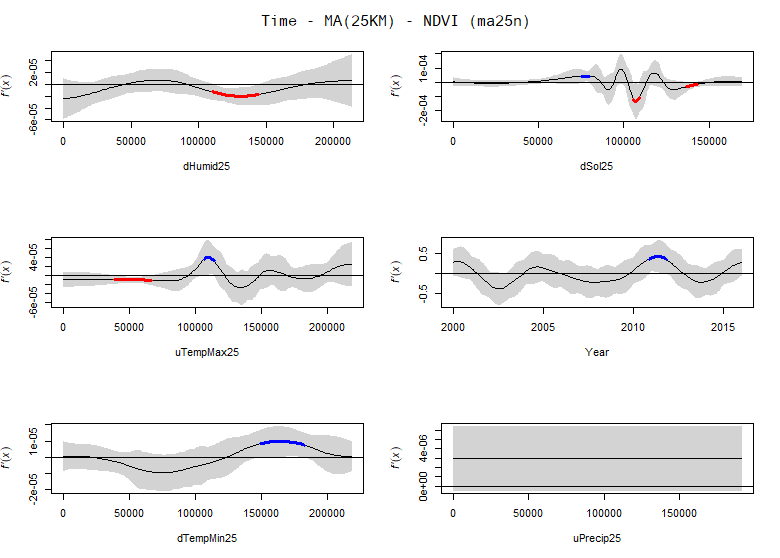
\includegraphics[width=1\textwidth]{ma25n.png} % first figure itself
        \caption{\textbf{Model ma25n}}
    \end{minipage}\hfill
    \begin{minipage}{0.8\textwidth}
        \centering
        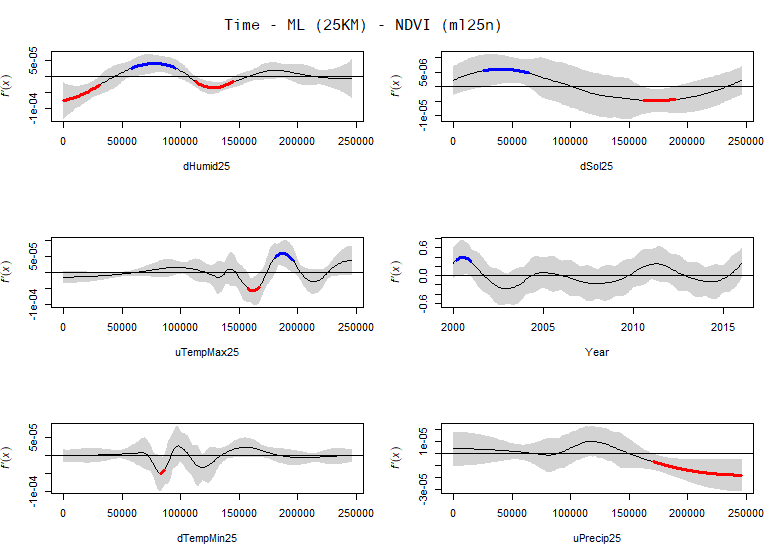
\includegraphics[width=1\textwidth]{ml25n.png} % second figure itself
        \caption{\textbf{Model ml25n}}
    \end{minipage}
\end{figure}

\begin{figure}[H]
 \centering
    \begin{minipage}{0.8\textwidth}
        \centering
        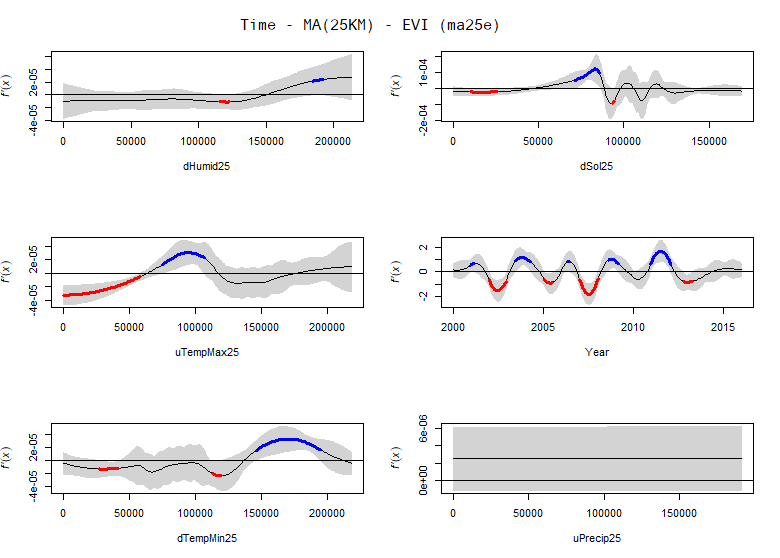
\includegraphics[width=1.2\textwidth]{ma25e.png} % first figure itself
        \caption{\textbf{Model ma25e}}
    \end{minipage}\hfill
    \begin{minipage}{0.8\textwidth}
        \centering
        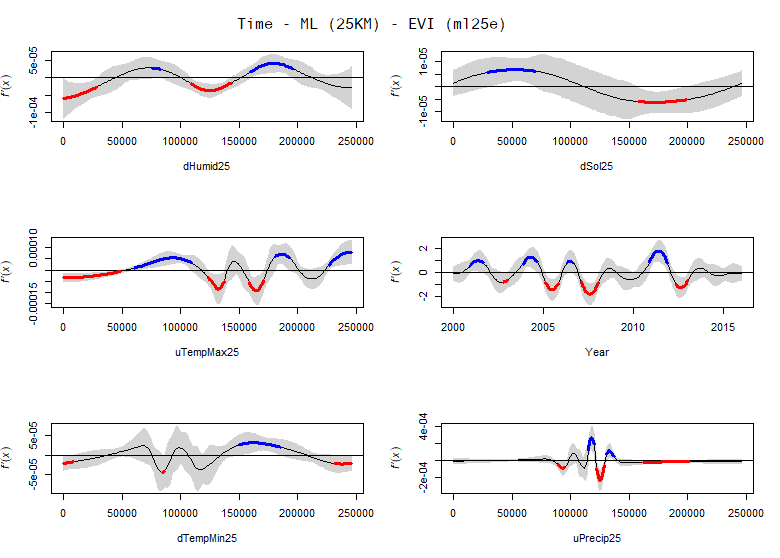
\includegraphics[width=1.2\textwidth]{ml25e.png} % second figure itself
        \caption{\textbf{Model ml25e}}
    \end{minipage}
\end{figure}

\begin{comment}
\begin{figure}[H]

    \begin{minipage}{0.8\textwidth}
        \centering
        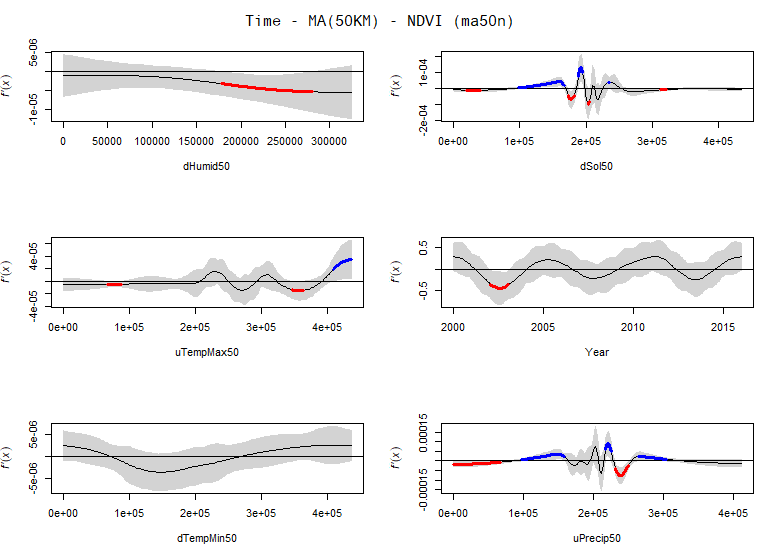
\includegraphics[width=1.2\textwidth]{ma50n.png} % first figure itself
        \caption{\textbf{Model ma50n}}
    \end{minipage}\hfill
    \begin{minipage}{0.8\textwidth}
        \centering
        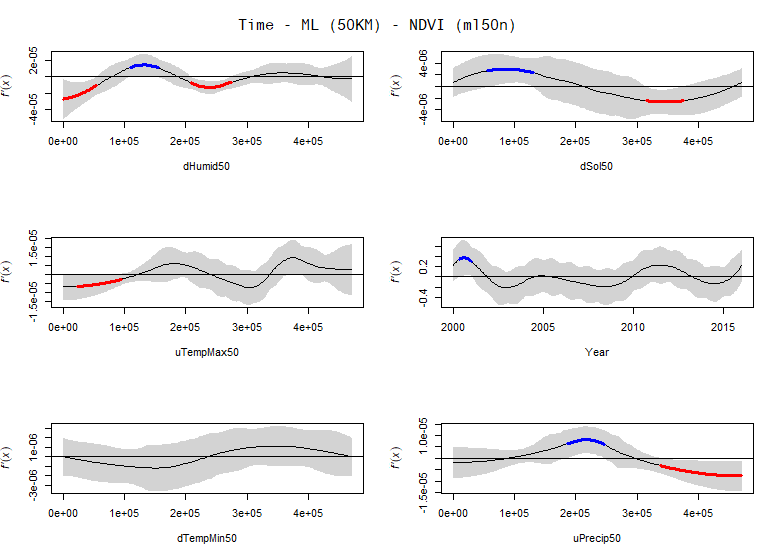
\includegraphics[width=1.2\textwidth]{ml50n.png} % second figure itself
        \caption{\textbf{Model ml50n}}
    \end{minipage}
\end{figure}

\begin{figure}[H]
 \centering
    \begin{minipage}{0.8\textwidth}
        \centering
        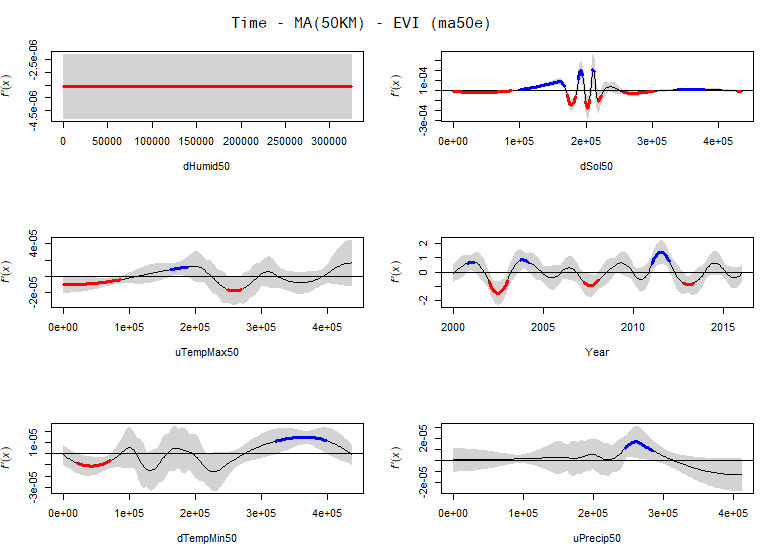
\includegraphics[width=1.2\textwidth]{ma50e.png} % first figure itself
        \caption{\textbf{Model ma50e}}
    \end{minipage}\hfill
    \begin{minipage}{0.8\textwidth}
        \centering
        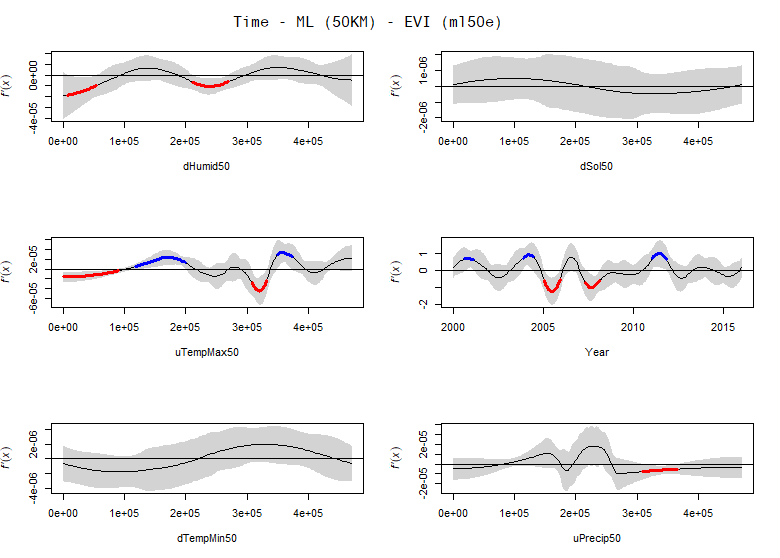
\includegraphics[width=1.2\textwidth]{ml50e.png} % second figure itself
        \caption{\textbf{Model ml50e}}
    \end{minipage}
\end{figure}

\begin{figure}[H]
    \begin{minipage}{0.8\textwidth}
        \centering
        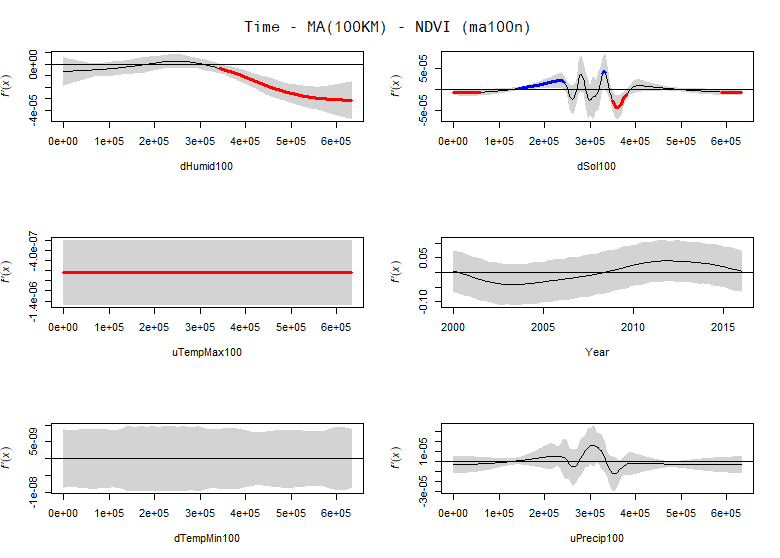
\includegraphics[width=1.2\textwidth]{ma100n.png} % first figure itself
        \caption{\textbf{Model ma100n}}
    \end{minipage}\hfill
    \begin{minipage}{0.8\textwidth}
        \centering
        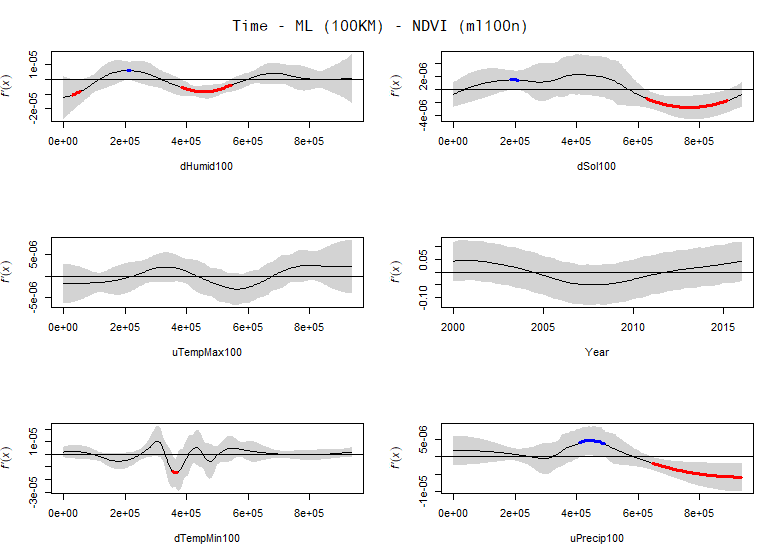
\includegraphics[width=1.2\textwidth]{ml100n.png} % second figure itself
        \caption{\textbf{Model ml100n}}
    \end{minipage}
\end{figure}

\begin{figure}[H]
 \centering
    \begin{minipage}{0.8\textwidth}
        \centering
        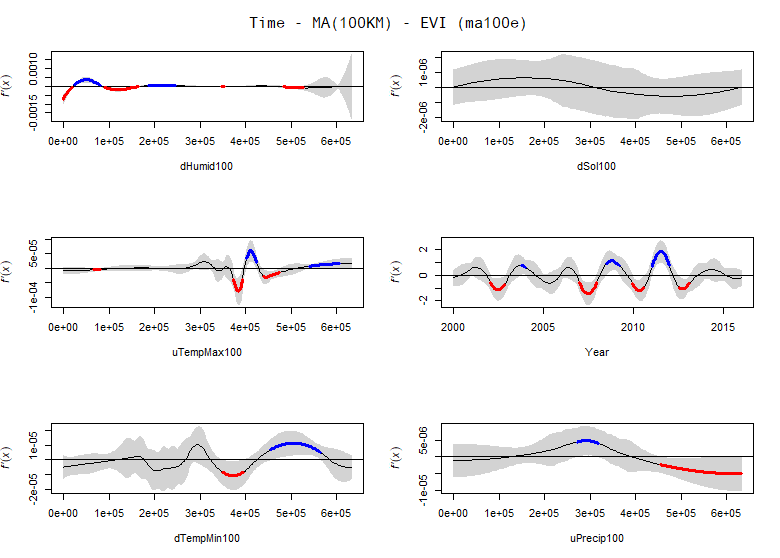
\includegraphics[width=1.2\textwidth]{ma100e.png} % first figure itself
        \caption{\textbf{Model ma100e}}
    \end{minipage}\hfill
    \begin{minipage}{0.8\textwidth}
        \centering
        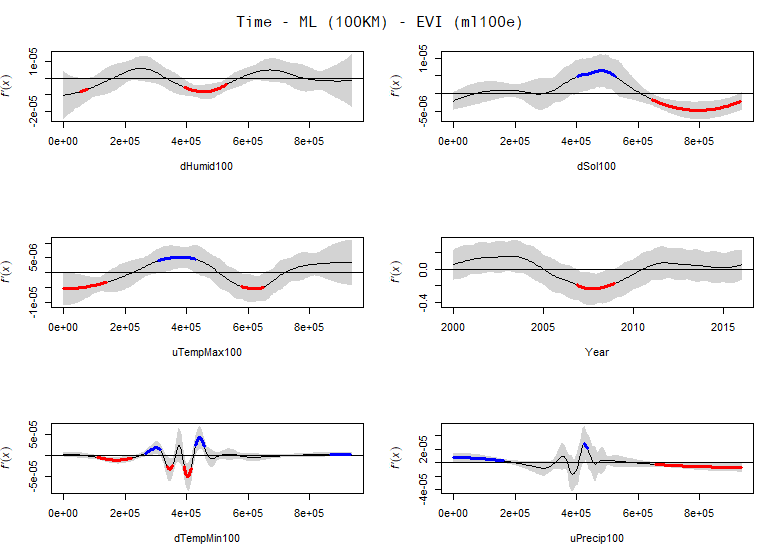
\includegraphics[width=1.2\textwidth]{ml100e.png} % second figure itself
        \caption{\textbf{Model ml100e}}
    \end{minipage}
\end{figure}
\end{comment}

\begin{figure}[H]
 \centering
    \begin{minipage}{0.8\textwidth}
        \centering
        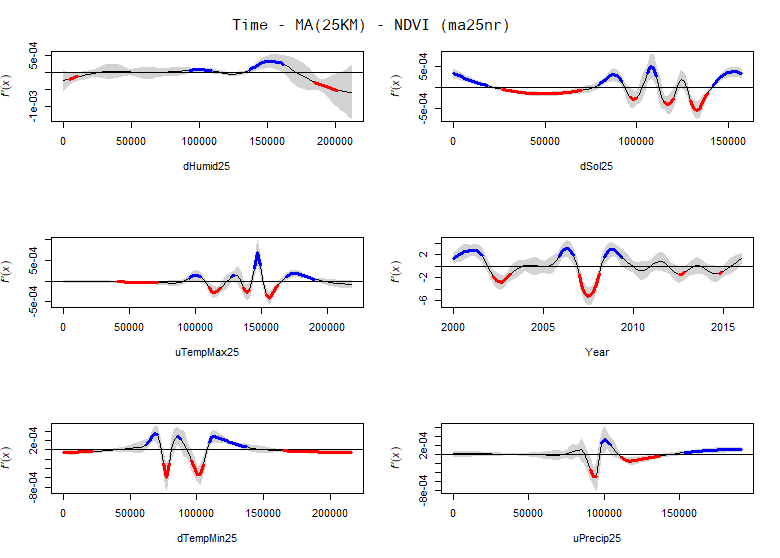
\includegraphics[width=1.2\textwidth]{ma25nr.png} % first figure itself
        \caption{\textbf{Model ma25nr}}
    \end{minipage}\hfill
    \begin{minipage}{0.8\textwidth}
        \centering
        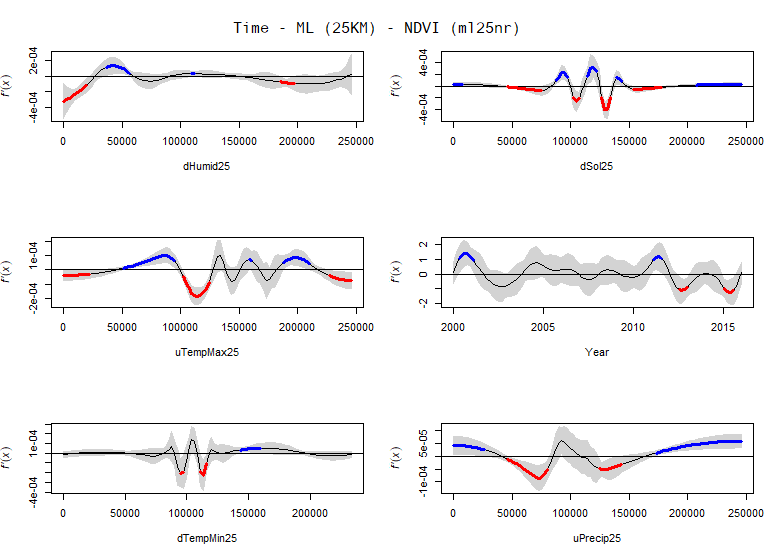
\includegraphics[width=1.2\textwidth]{ml25nr.png} % second figure itself
        \caption{\textbf{Model ml25nr}}
    \end{minipage}
\end{figure}

\begin{figure}[H]
 \centering
    \begin{minipage}{0.8\textwidth}
        \centering
        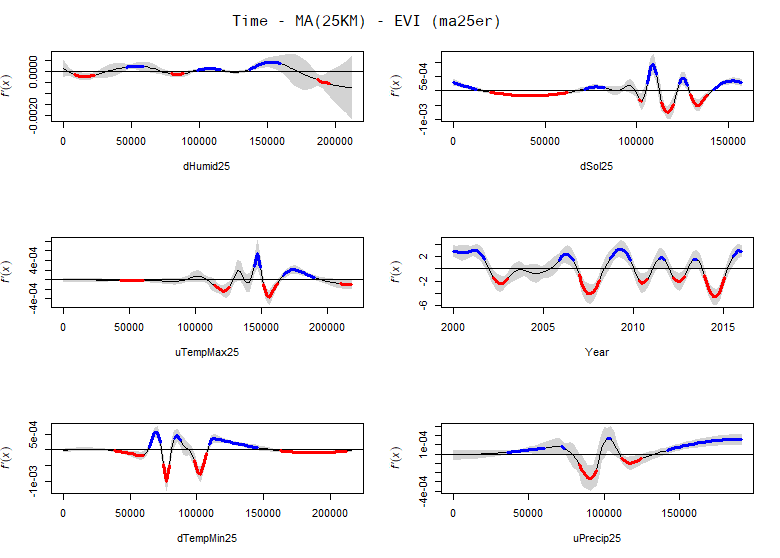
\includegraphics[width=1.2\textwidth]{ma25er.png} % first figure itself
        \caption{\textbf{Model ma25er}}
    \end{minipage}\hfill
    \begin{minipage}{0.8\textwidth}
        \centering
        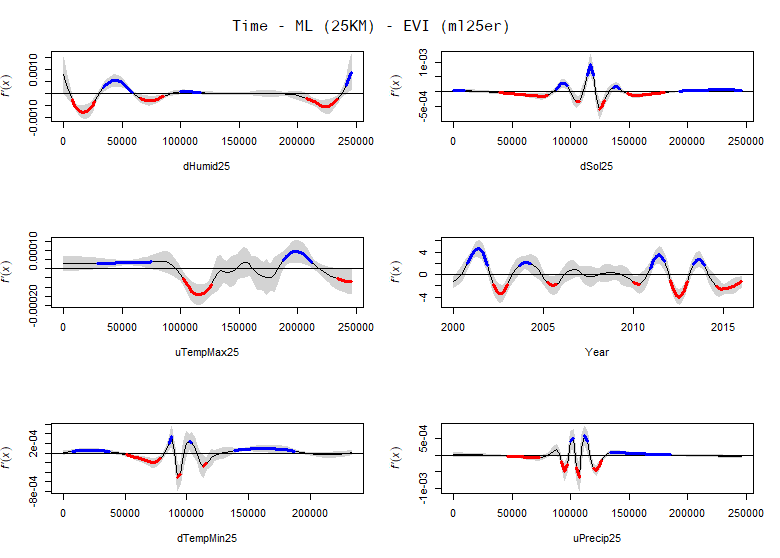
\includegraphics[width=1.2\textwidth]{ml25er.png} % second figure itself
        \caption{\textbf{Model ml25er}}
    \end{minipage}
\end{figure}

\begin{figure}[H]

    \begin{minipage}{0.8\textwidth}
        \centering
        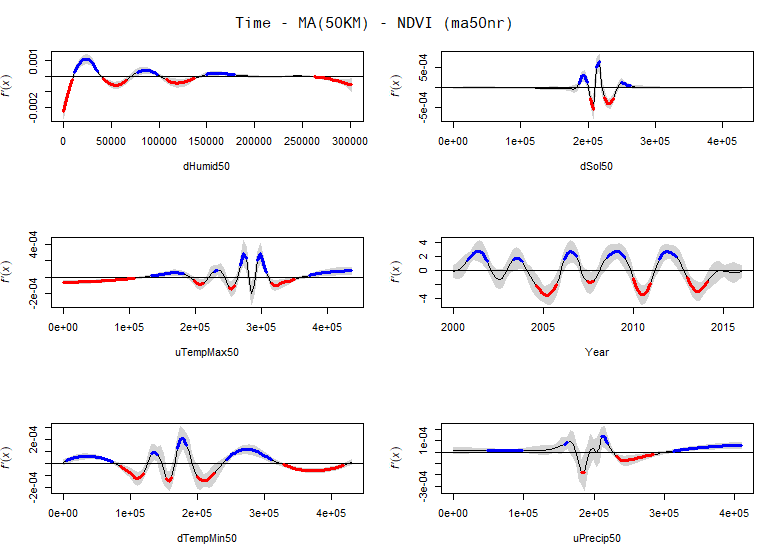
\includegraphics[width=1.2\textwidth]{ma50nr.png} % first figure itself
        \caption{\textbf{Model ma50nr}}
    \end{minipage}\hfill
    \begin{minipage}{0.8\textwidth}
        \centering
        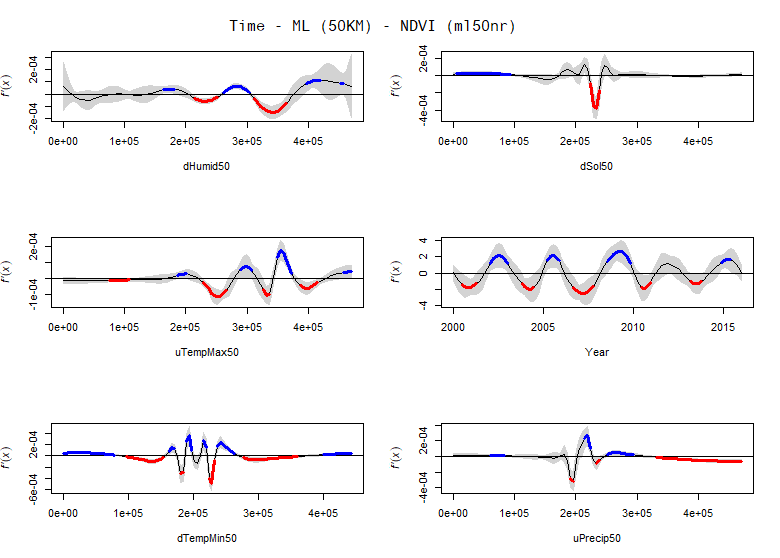
\includegraphics[width=1.2\textwidth]{ml50nr.png} % second figure itself
        \caption{\textbf{Model ml50nr}}
    \end{minipage}
\end{figure}

\begin{figure}[H]
 \centering
    \begin{minipage}{0.8\textwidth}
        \centering
        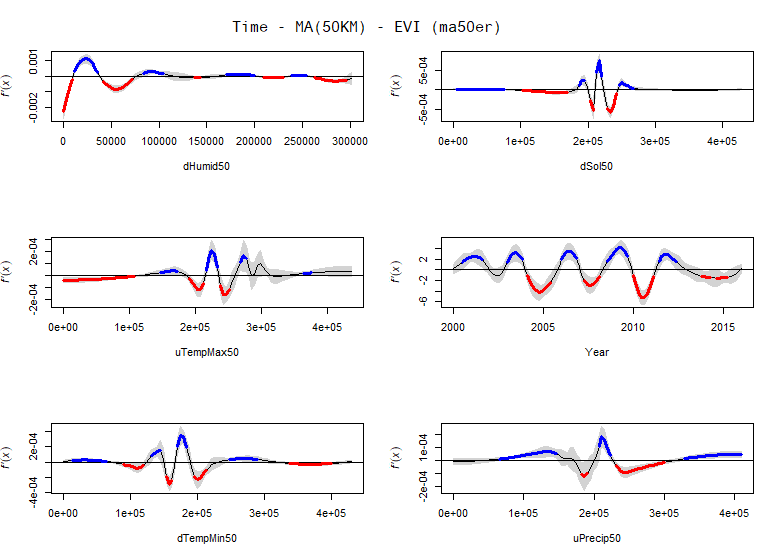
\includegraphics[width=1.2\textwidth]{ma50er.png} % first figure itself
        \caption{\textbf{Model ma50er}}
    \end{minipage}\hfill
    \begin{minipage}{0.8\textwidth}
        \centering
        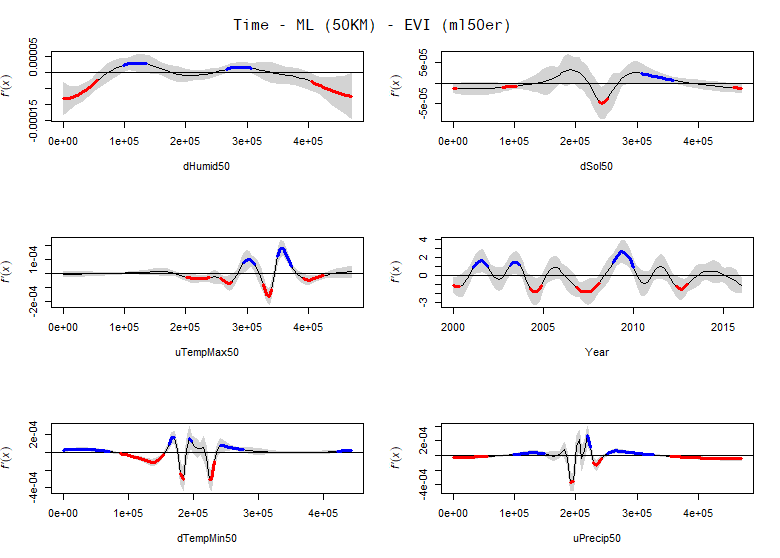
\includegraphics[width=1.2\textwidth]{ml50er.png} % second figure itself
        \caption{\textbf{Model ml50er}}
    \end{minipage}
\end{figure}

\begin{figure}[H]
    \begin{minipage}{0.8\textwidth}
        \centering
        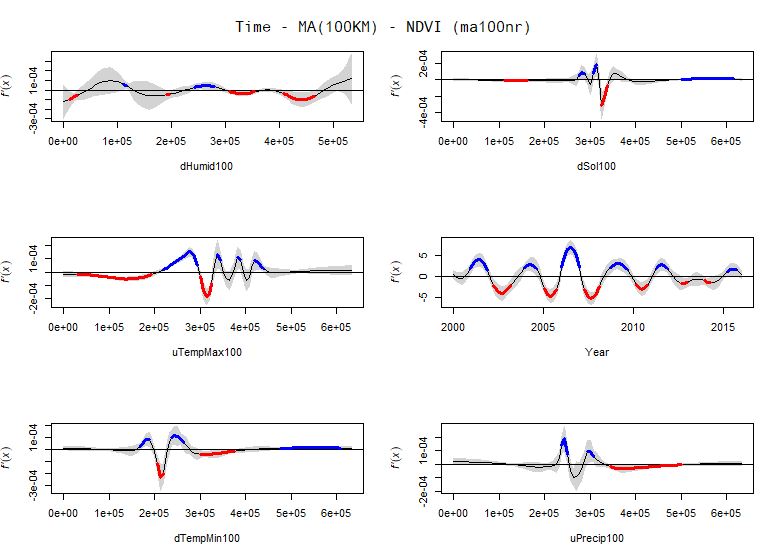
\includegraphics[width=1.2\textwidth]{ma100nr.png} % first figure itself
        \caption{\textbf{Model ma100nr}}
    \end{minipage}\hfill
    \begin{minipage}{0.8\textwidth}
        \centering
        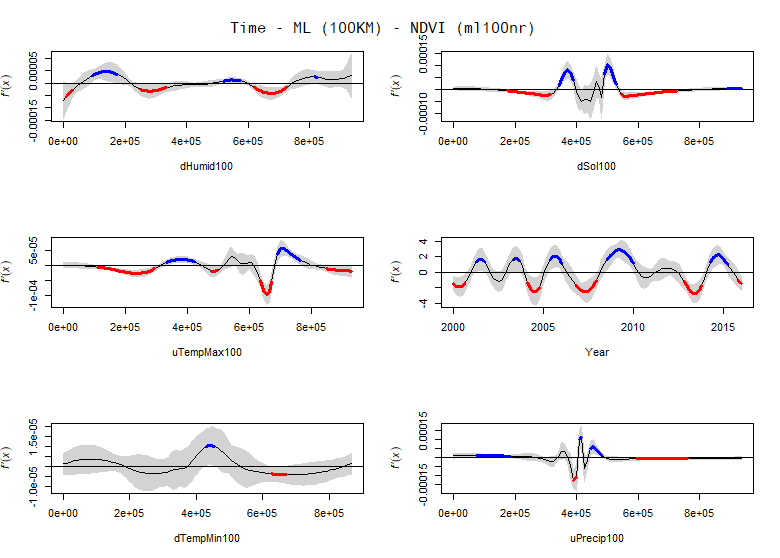
\includegraphics[width=1.2\textwidth]{ml100nr.png} % second figure itself
        \caption{\textbf{Model ml100nr}}
    \end{minipage}
\end{figure}

\begin{figure}[H]
 \centering
    \begin{minipage}{0.8\textwidth}
        \centering
        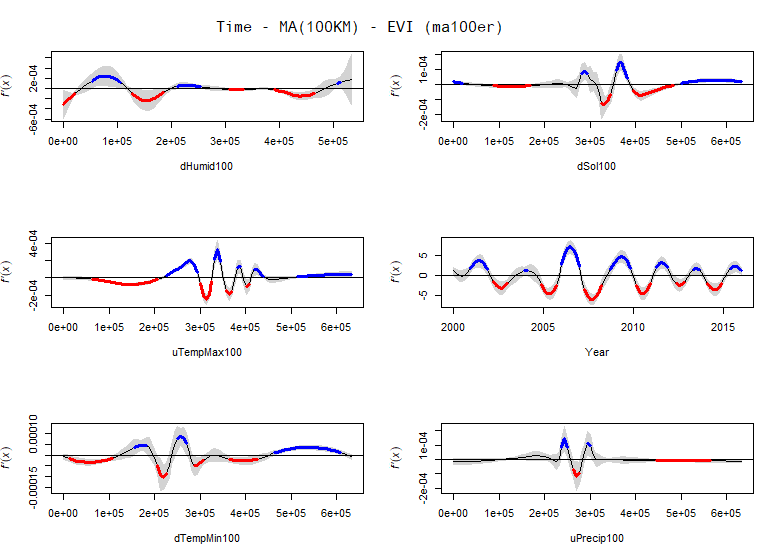
\includegraphics[width=1.2\textwidth]{ma100er.png} % first figure itself
        \caption{\textbf{Model ma100er}}
    \end{minipage}\hfill
    \begin{minipage}{0.8\textwidth}
        \centering
        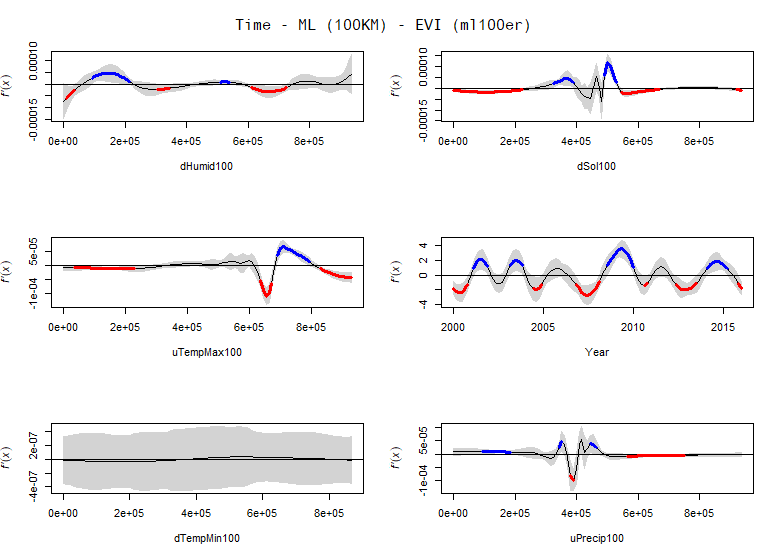
\includegraphics[width=1.2\textwidth]{ml100er.png} % second figure itself
        \caption{\textbf{Model ml100er}}
    \end{minipage}
\end{figure}

\begin{figure}[H]
 \centering
    \begin{minipage}{0.8\textwidth}
        \centering
        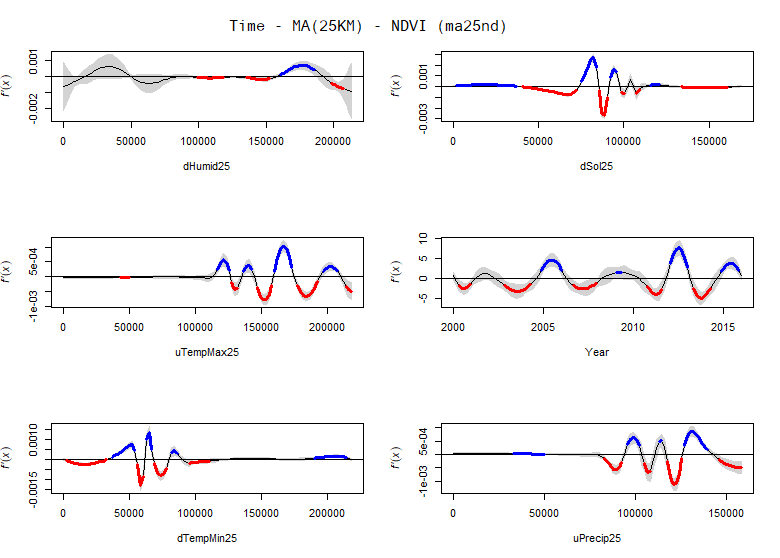
\includegraphics[width=1.2\textwidth]{ma25nd.png} % first figure itself
        \caption{\textbf{Model ma25nd}}
    \end{minipage}\hfill
    \begin{minipage}{0.8\textwidth}
        \centering
        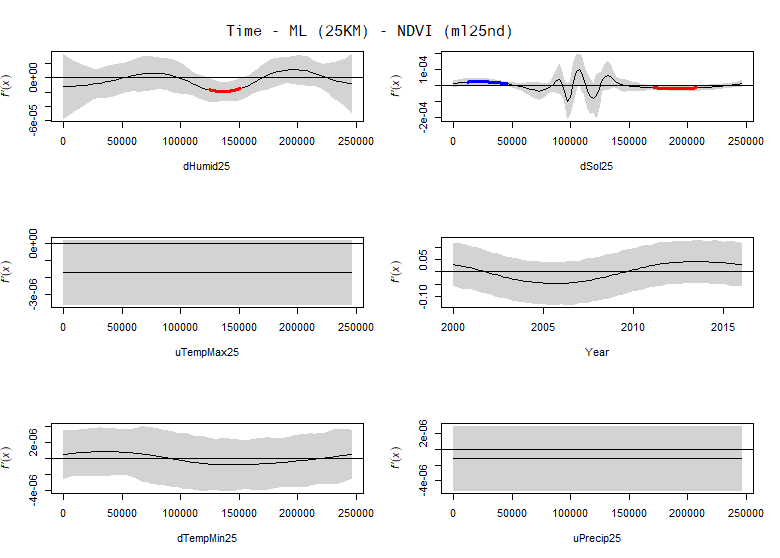
\includegraphics[width=1.2\textwidth]{ml25nd.png} % second figure itself
        \caption{\textbf{Model ml25nd}}
    \end{minipage}
\end{figure}

\begin{figure}[H]
 \centering
    \begin{minipage}{0.8\textwidth}
        \centering
        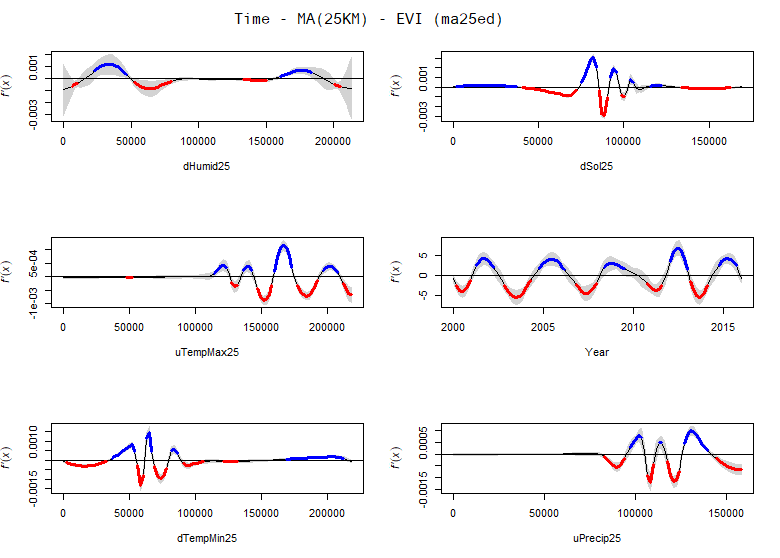
\includegraphics[width=1.2\textwidth]{ma25ed.png} % first figure itself
        \caption{\textbf{Model ma25ed}}
    \end{minipage}\hfill
    \begin{minipage}{0.8\textwidth}
        \centering
        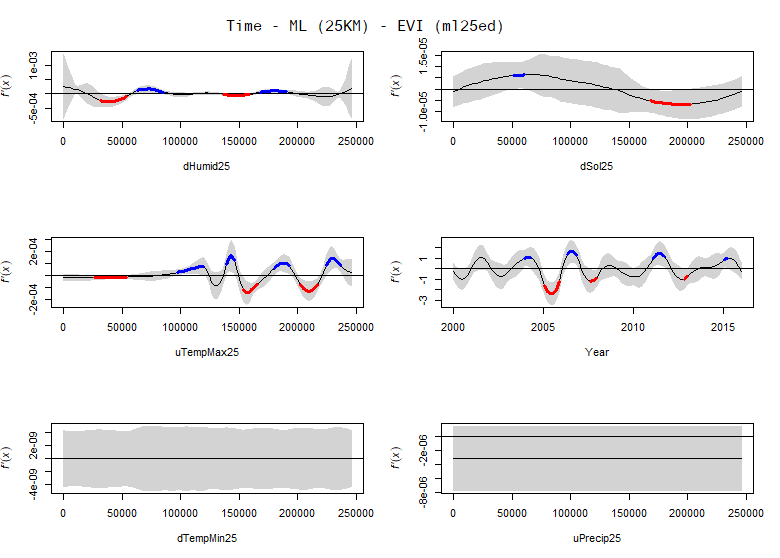
\includegraphics[width=1.2\textwidth]{ml25ed.png} % second figure itself
        \caption{\textbf{Model ml25ed}}
    \end{minipage}
\end{figure}

\begin{figure}[H]

    \begin{minipage}{0.8\textwidth}
        \centering
        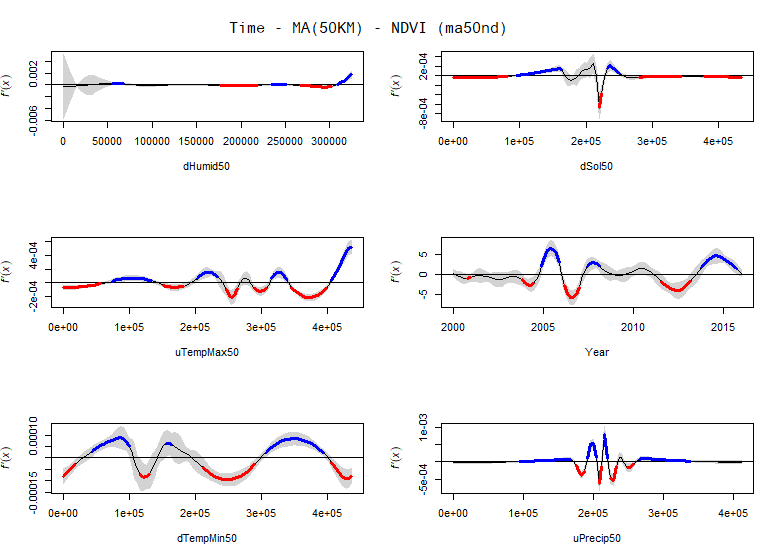
\includegraphics[width=1.2\textwidth]{ma50nd.png} % first figure itself
        \caption{\textbf{Model ma50nd}}
    \end{minipage}\hfill
    \begin{minipage}{0.8\textwidth}
        \centering
        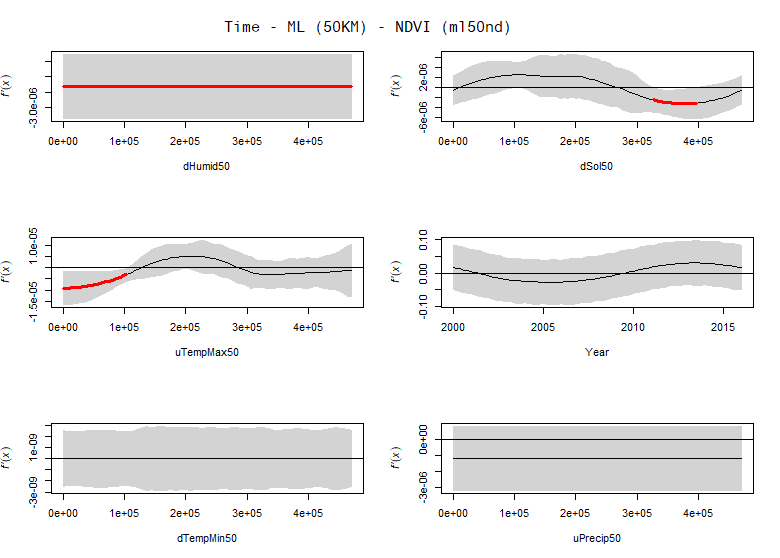
\includegraphics[width=1.2\textwidth]{ml50nd.png} % second figure itself
        \caption{\textbf{Model ml50nd}}
    \end{minipage}
\end{figure}

\begin{figure}[H]
 \centering
    \begin{minipage}{0.8\textwidth}
        \centering
        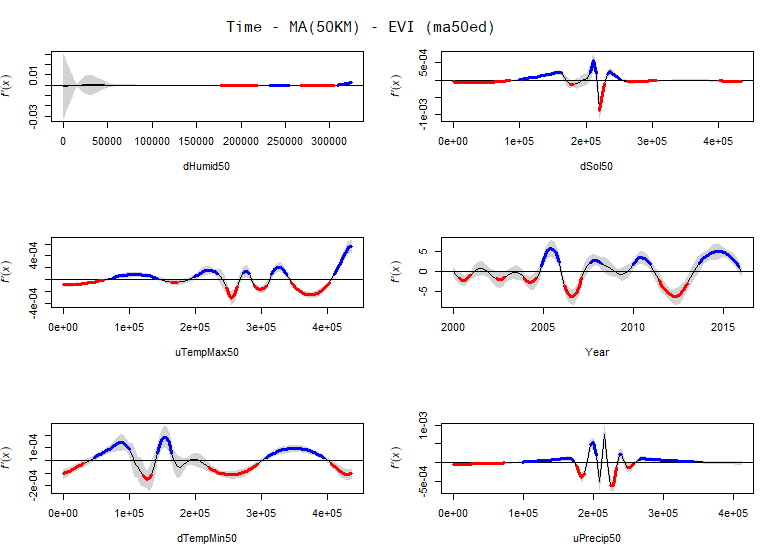
\includegraphics[width=1.2\textwidth]{ma50ed.png} % first figure itself
        \caption{\textbf{Model ma50ed}}
    \end{minipage}\hfill
    \begin{minipage}{0.8\textwidth}
        \centering
        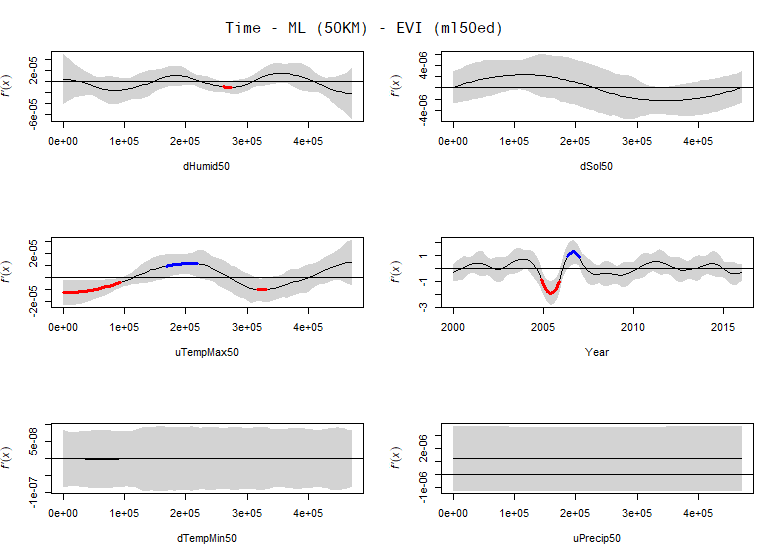
\includegraphics[width=1.2\textwidth]{ml50ed.png} % second figure itself
        \caption{\textbf{Model ml50ed}}
    \end{minipage}
\end{figure}

\begin{figure}[H]
    \begin{minipage}{0.8\textwidth}
        \centering
        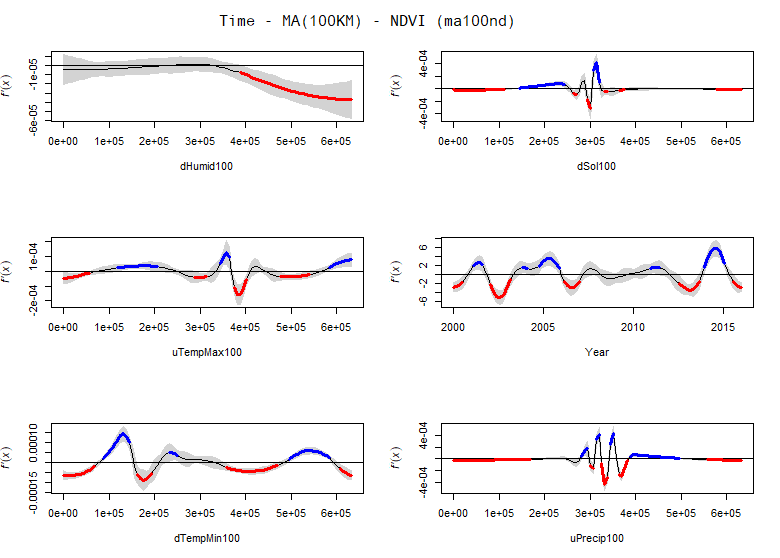
\includegraphics[width=1.2\textwidth]{ma100nd.png} % first figure itself
        \caption{\textbf{Model ma100nd}}
    \end{minipage}\hfill
    \begin{minipage}{0.8\textwidth}
        \centering
        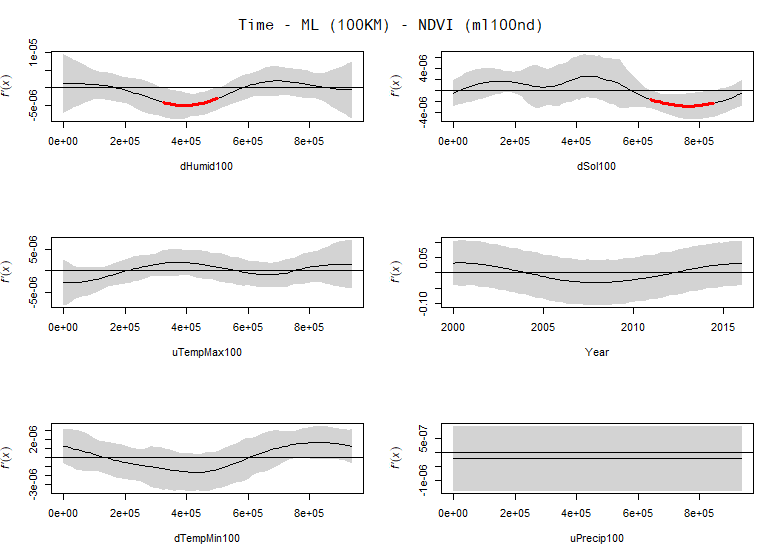
\includegraphics[width=1.2\textwidth]{ml100nd.png} % second figure itself
        \caption{\textbf{Model ml100nd}}
    \end{minipage}
\end{figure}

\begin{figure}[H]
 \centering
    \begin{minipage}{0.8\textwidth}
        \centering
        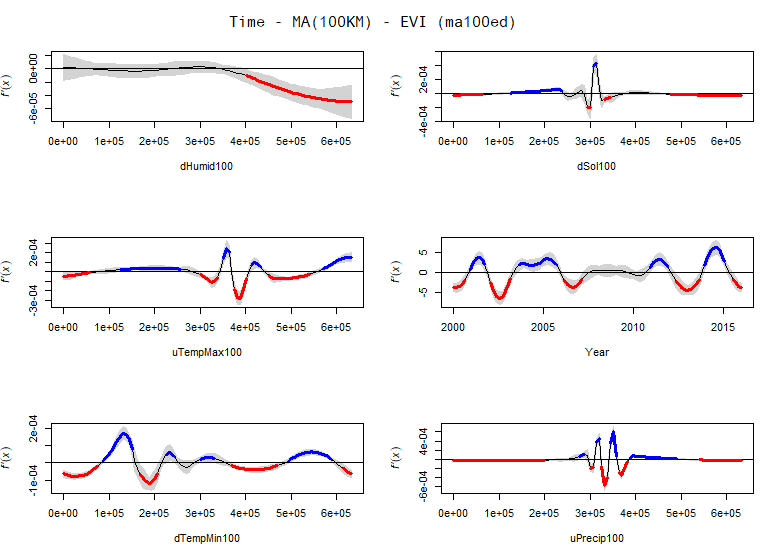
\includegraphics[width=1.2\textwidth]{ma100ed.png} % first figure itself
        \caption{\textbf{Model ma100ed}}
    \end{minipage}\hfill
    \begin{minipage}{0.8\textwidth}
        \centering
        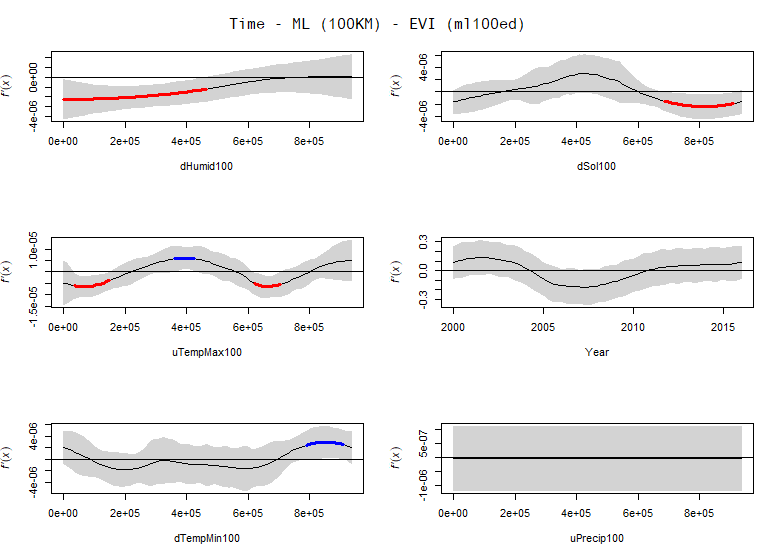
\includegraphics[width=1.2\textwidth]{ml100ed.png} % second figure itself
        \caption{\textbf{Model ml100ed}}
    \end{minipage}
\end{figure}


\begin{figure}[H]
  \centering
  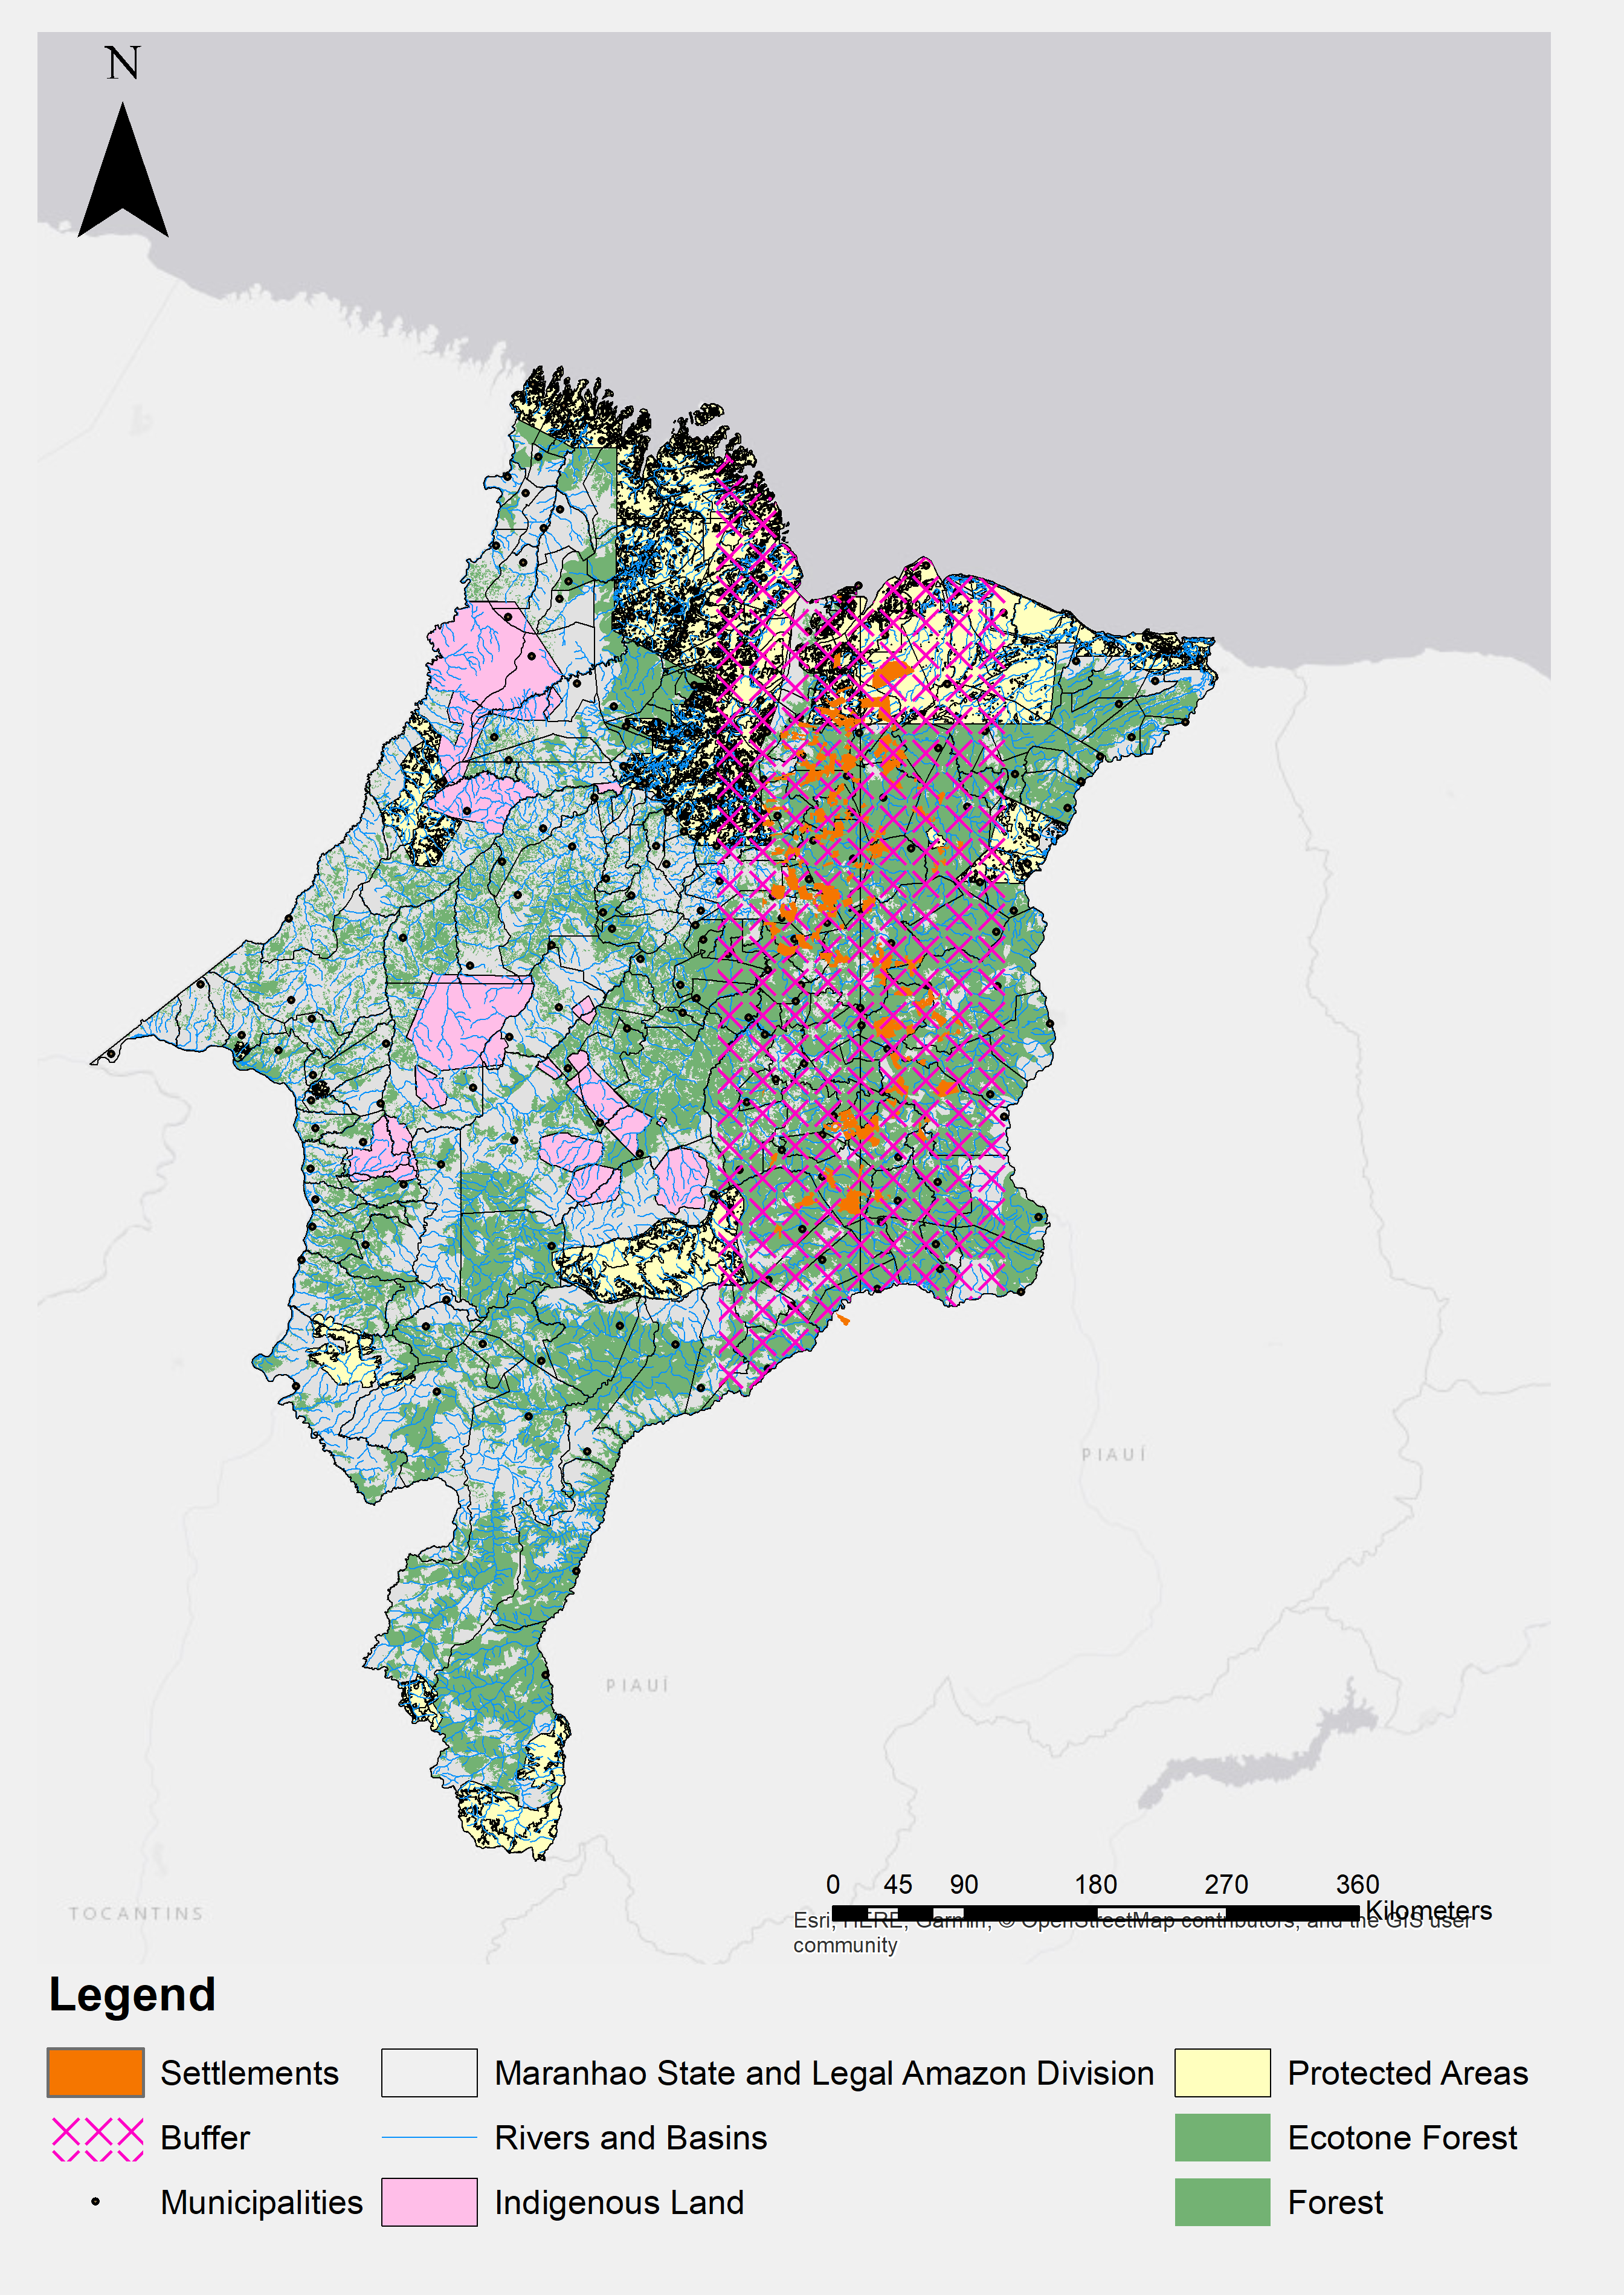
\includegraphics[width=1\textwidth, inner]{Chapter2/MaranhaoChapter2_Fig3.png}
\caption{Source: \citep{MMMAwebsite,nugeo_2018,embrapa_2018, INCRA}.}
\label{fig:delimitacaosett}
\end{figure}

\begin{landscape}
\begin{figure}[H]
  \centering
  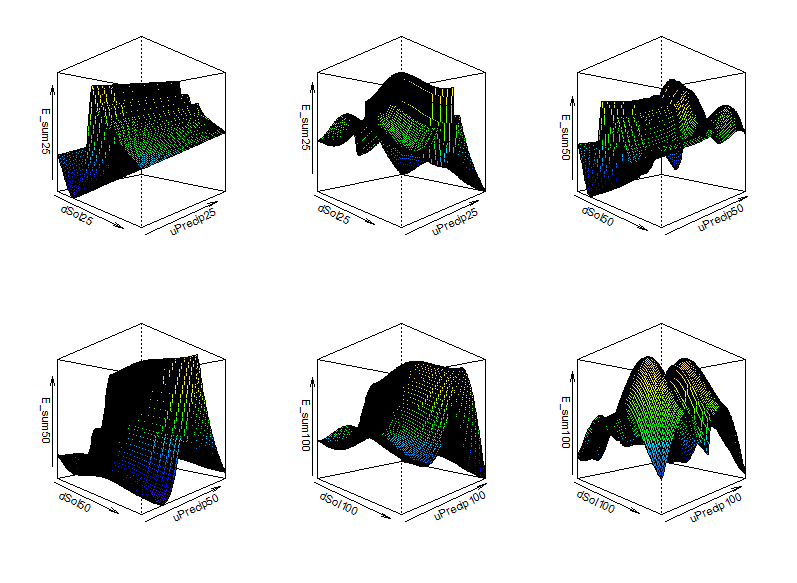
\includegraphics[width=1.5\textwidth, inner]{visgam.png}
\caption{\textbf{Interactions between selected variables for the baseline model.}}
\label{fig:visgam}
\end{figure}



\begin{figure}[H]
  \centering
  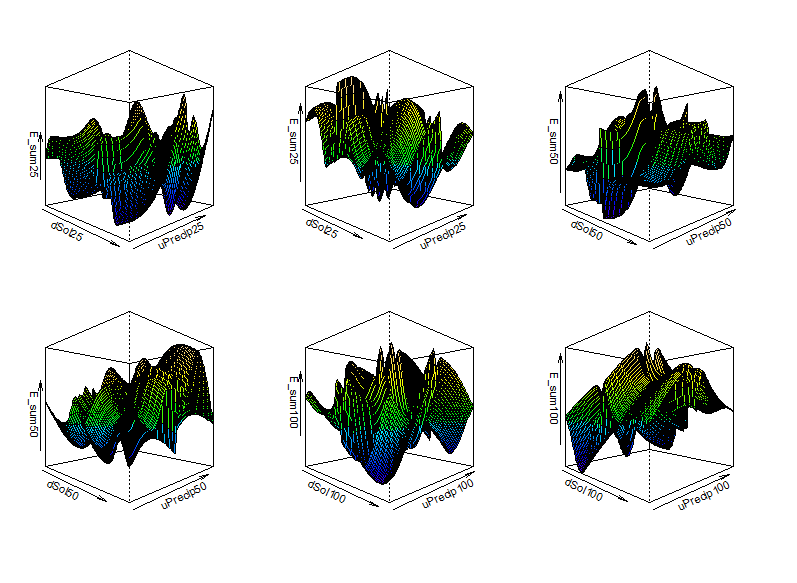
\includegraphics[width=1.5\textwidth, inner]{visgamr.png}
\caption{\textbf{Interactions between selected variables for the rain season model.}}
\label{fig:visgamr}
\end{figure}


\begin{figure}[H]
  \centering
  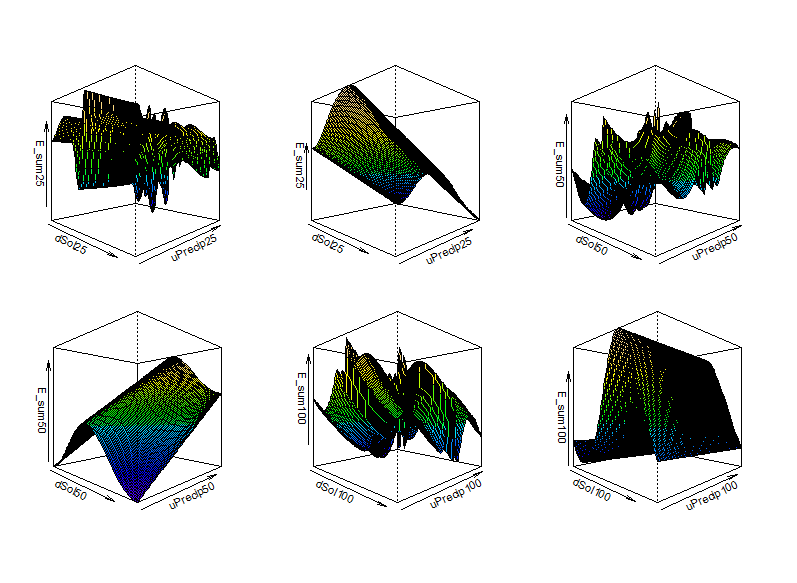
\includegraphics[width=1.5\textwidth, inner]{visgamd.png}
\caption{\textbf{Interactions between selected variables for the dry season model.}}
\label{fig:visgamd}
\end{figure}


\begin{figure}[H]
  \centering
  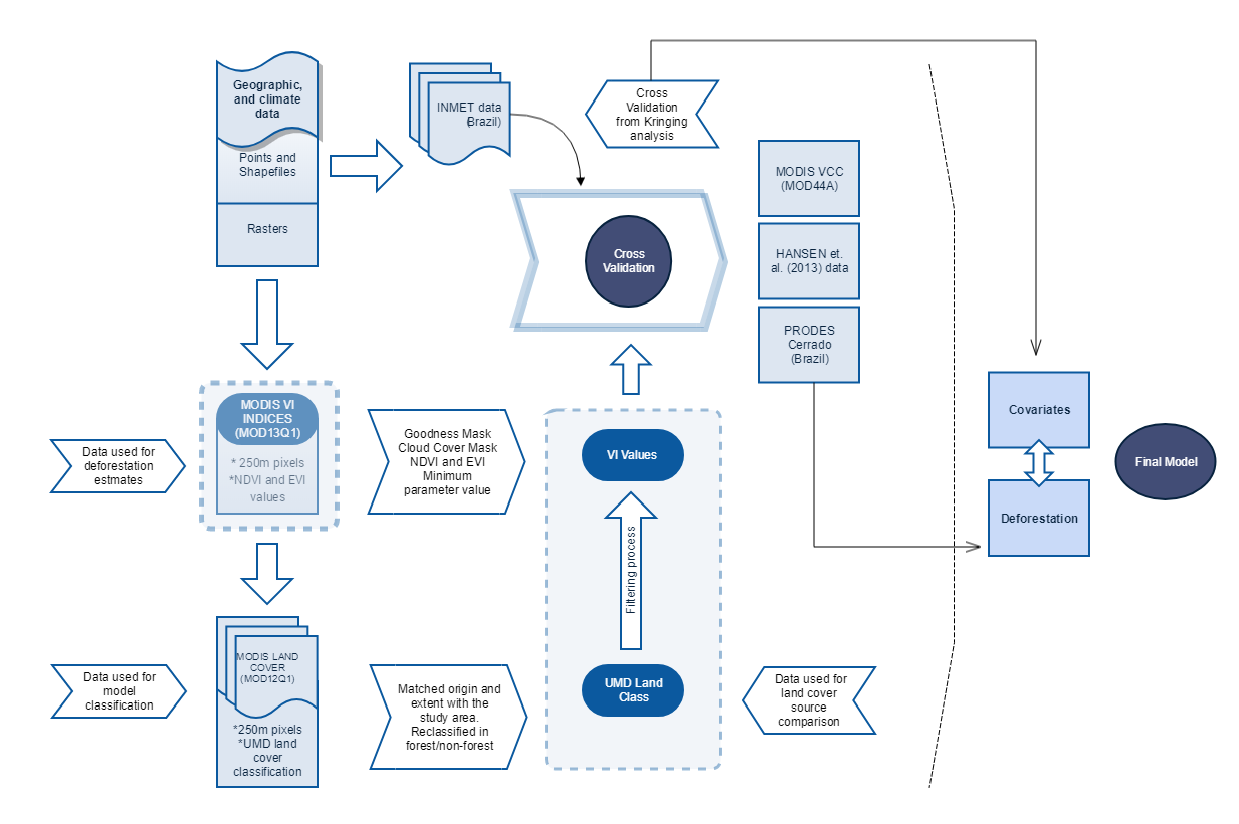
\includegraphics[width=1.5\textwidth, inner]{method.png}
\caption{\textbf{Flowchart of method applied to data}. Moving from left to right indicates increasing levels of data processing during the study.}
\label{fig:method}
\end{figure}
\end{landscape}

\end{appendices}
